% This is a LaTeX thesis template for Adam Mickiewicz University.
% to be used with Rmarkdown
% This template was produced by Jakub Nowosad
% Version: 16 February 2020

% Inspired by:
% This is a LaTeX thesis template for Monash University.
% to be used with Rmarkdown
% This template was produced by Rob Hyndman
% Version: 6 September 2016

\documentclass{amuthesis}
%\usepackage[polish]{babel}
%\usepackage{polski}
%\renewcommand{\figurename}{Figure} % Redefine default figure caption %
%\renewcommand{\tablename}{Table} % Redefine default table caption %
%%%%%%%%%%%%%%%%%%%%%%%%%%%%%%%%%%%%%%%%%%%%%%%%%%%%%%%%%%%%%%%
% Add any LaTeX packages and other preamble here if required
%%%%%%%%%%%%%%%%%%%%%%%%%%%%%%%%%%%%%%%%%%%%%%%%%%%%%%%%%%%%%%%
\usepackage{booktabs,tabularx} % Allows kableExtra to work %
\usepackage{indentfirst} % Adds indent in the first paragraph %
\usepackage{bookmark} % Adds indent in the first paragraph %
\usepackage{booktabs}
\usepackage{longtable}
\usepackage{array}
\usepackage{multirow}
\usepackage{wrapfig}
\usepackage{float}
\usepackage{colortbl}
\usepackage{pdflscape}
\usepackage{tabu}
\usepackage{threeparttable}
\usepackage{threeparttablex}
\usepackage[normalem]{ulem}
\usepackage{makecell}
\usepackage{xcolor}

\author{Tomasz Matuszek}
\title{Measuring an impact of the Landsat 8 thermal band on the
supervised land cover classification results}
\def\titleeng{Ocena wpływu zastosowania kanału termalnego Landsat 8 na
wyniki nadzorowanej klasyfikacji pokrycia terenu}
\def\degreetitle{Engineer's thesis}
\def\major{Geoinformation}
\def\albumid{455828}
\def\thesisyear{2023}
% Add subject and keywords below
\hypersetup{
     %pdfsubject={The Subject},
     %pdfkeywords={Some Keywords},
     pdfauthor={Tomasz Matuszek},
     pdftitle={Measuring an impact of the Landsat 8 thermal band on the
supervised land cover classification results},
     pdfproducer={quarto with LaTeX}
}

\bibliography{thesis,packages}

\begin{document}

\pagenumbering{arabic}

\titlepage

\bookmarksetup{startatroot}

\hypertarget{abstract}{%
\chapter*{Abstract}\label{abstract}}
\addcontentsline{toc}{chapter}{Abstract}

\markboth{Abstract}{Abstract}

\textbf{Abstract}

Accurate land cover maps are crucial in many fields of geography, urban
planning and environmental studies. Currently, the most popular method
to create such maps is the usage of machine learning techniques and
satellite imagery. Researchers still investigate different variables and
approaches in strive to achieve the highest possible accuracy of their
predictions. The goal of this study was to evaluate importance of
thermal band acquired from Landsat 8 programme for land cover mapping.
LUCAS land cover reference dataset was used to fit the Random Forest
model. Apart from training the model, several machine learning
techniques such as hyperparameter tuning, nested spatial
cross-validation and benchmarking were performed in order to achieve
possibly high and accurate performance measures. Moreover, thermal
band's importance on model results was investigated. Analysis of the
variable importance showed that impact of the land surface temperature
was not very high, but indeed visible. Moreover, I discovered that
thermal band had significantly higher impact on the model prediction
when classifying artificial land. These findings suggest that thermal
information may be influential in the mapping development of urban
areas. However, further studies involving spatio-temporal analysis for
more study areas are needed to quantify thermal band's impact more
precisely.

Keywords: machine learning, remote sensing, variable importance, land
surface temperature

\newpage

\textbf{Abstrakt}

Dokładne mapy pokrycia terenu mają kluczowe znaczenie w wielu
dziedzinach geografii, urbanistyki i badań środowiskowych. W ostatnich
latach najpopularniejszą metodą tworzenia takich map jest wykorzystanie
zobrazowań satelitarnych oraz technik uczenia maszynowego. Naukowcy
wciąż badają zastosowanie różnych zmiennych i podejść, dążąc do
osiągnięcia jak najwyższej dokładności swoich modeli. Celem niniejszej
pracy była ocena znaczenia kanału termalnego pozyskanego z satelity
Landsat 8 w tworzeniu map pokrycia terenu. Do stworzenia modelu lasu
losowego wykorzystano zbiór danych o pokryciu terenu pozyskany w ramach
programu LUCAS. Poza treningiem modelu, w celu uzyskania możliwie
wysokiej jakości modelu i dokładnej jego oceny, zastosowano techniki
uczenia maszynowego, takie jak optymalizacja parametrów, kroswalidacja
przestrzenna oraz benchmarking. Ponadto, zbadano znaczenie kanału
termalnego na wyniki modelu. Analiza istotności zmiennych wykazała, że
wpływ temperatury nie był wysoki, ale widoczny. Co więcej zauważono, że
kanał termalny miał znacząco większy wpływ na wyniki modelu dla
klasyfikacji obszarów zabudowanych. Wyniki te sugerują, że informacja
termiczna może mieć wpływ na lepsze mapowanie rozwoju obszarów
miejskich. Jednakże aby dokładniej określić wpływ kanału termalnego,
potrzebne są dalsze badania obejmujące analizę przestrzenno-czasową dla
większej liczby obszarów badawczych.

Słowa kluczowe: uczenie maszynowe, teledetekcja, istotność zmiennych,
temperatura powierzchni

\newpage

\setstretch{1.2}\sf\tighttoc\doublespacing

\bookmarksetup{startatroot}

\hypertarget{sec-intro}{%
\chapter{Introduction}\label{sec-intro}}

Land cover is a physical characteristic of Earth's surface describing
distribution of vegetation, water, soil and other features on the ground
\autocite{rawat_monitoring_2015}. The production of accurate land cover
maps is crucial for conducting spatial analyses, studying environmental
changes \autocite{reis_analyzing_2008} and evaluating urban development
\autocite{hashem_change_2015}. Land cover information is also useful for
the general circulation models (GCM) development
\autocite{running_ecosystem_2008} and has been selected as one of the
most essential variables that contribute to describing Earth's
environment and climate \autocite{bojinski_concept_2014}.

The main method of creating land cover maps is based on multispectral
satellite data and remote-sensing methods. The two most popular,
free-of-charge sources of satellite imagery are Landsat programme (run
by NASA and USGS) and Sentinel programme (conducted by ESA). These
datasets are usually utilized to create classification models based on
machine learning techniques, which gained popularity in the recent years
\autocite{maxwell_implementation_2018}. A supervised machine learning
model, including the one used in this study, analyzes training set
containing labels of land cover classes and tries to learn how to
recognize them.

Over the past few years, there were several attempts to automate
creation of land cover maps
\autocite{malinowski_automated_2020,witjes_spatiotemporal_2021}. An
automated workflow, however, requires high understanding of every step
of machine learning process and appropriate choice of explanatory
variables. Spectral bands and spectral indices are the most commonly
used variables. However, some satellites like Landsat 8, have a thermal
sensor as well, which measures land surface temperature (LST) of the
Earth. There is a significant interaction between LST and extent of
urban and impervious areas \autocite{dutta_changing_2019}, thus we can
assume that this variable might be influential on the classification
model results. Thermal band's impact on the model results is described
in several studies, for example,
\textcite{rodriguez-galiano_incorporating_2012},
\textcite{zhao_exploring_2019}, \textcite{sun_improvement_2015}.
However, despite adding completely new information compared to spectral
bands, the thermal band is noticeably more often omitted in
classification models, probably due to its coarser resolution
\autocite{rodriguez-galiano_incorporating_2012}. Because of this, its
impact on model predictions is not clear enough and needs further
research.

The main goal of this study is to evaluate thermal band's impact on a
classification model, study its spatial distribution and try to give
broader knowledge of how it should be used. Random Forest model will be
trained on a dataset for Poland and a land cover map of Poznań
metropolitan area will be created. Then, both the machine learning model
and the result map will be used to measure thermal band's impact on the
classification results.

\bookmarksetup{startatroot}

\hypertarget{sec-data-methods}{%
\chapter{Materials and methods}\label{sec-data-methods}}

Workflow of the study consisted of several stages: preprocessing of
source data (described in Sections \ref{sec-sat} and
\ref{sec-landcover}), creating a training dataset, model parameters
tuning and model quality assessment (Section~\ref{sec-resampling}), land
cover map prediction and evaluating the impact of the thermal band on
the model results (Section~\ref{sec-importance}). Visual representation
of the workflow is shown in Figure~\ref{fig-rycina1}.

Each of these steps was performed using R programming language
\autocite{R-base} and final visualizations were created in QGIS software
\autocite{qgis_development_team_qgis_2009}. Both programming environment
and GIS software used in this process are open-source.

\begin{figure}

{\centering 

\begin{figure}[H]

{\centering 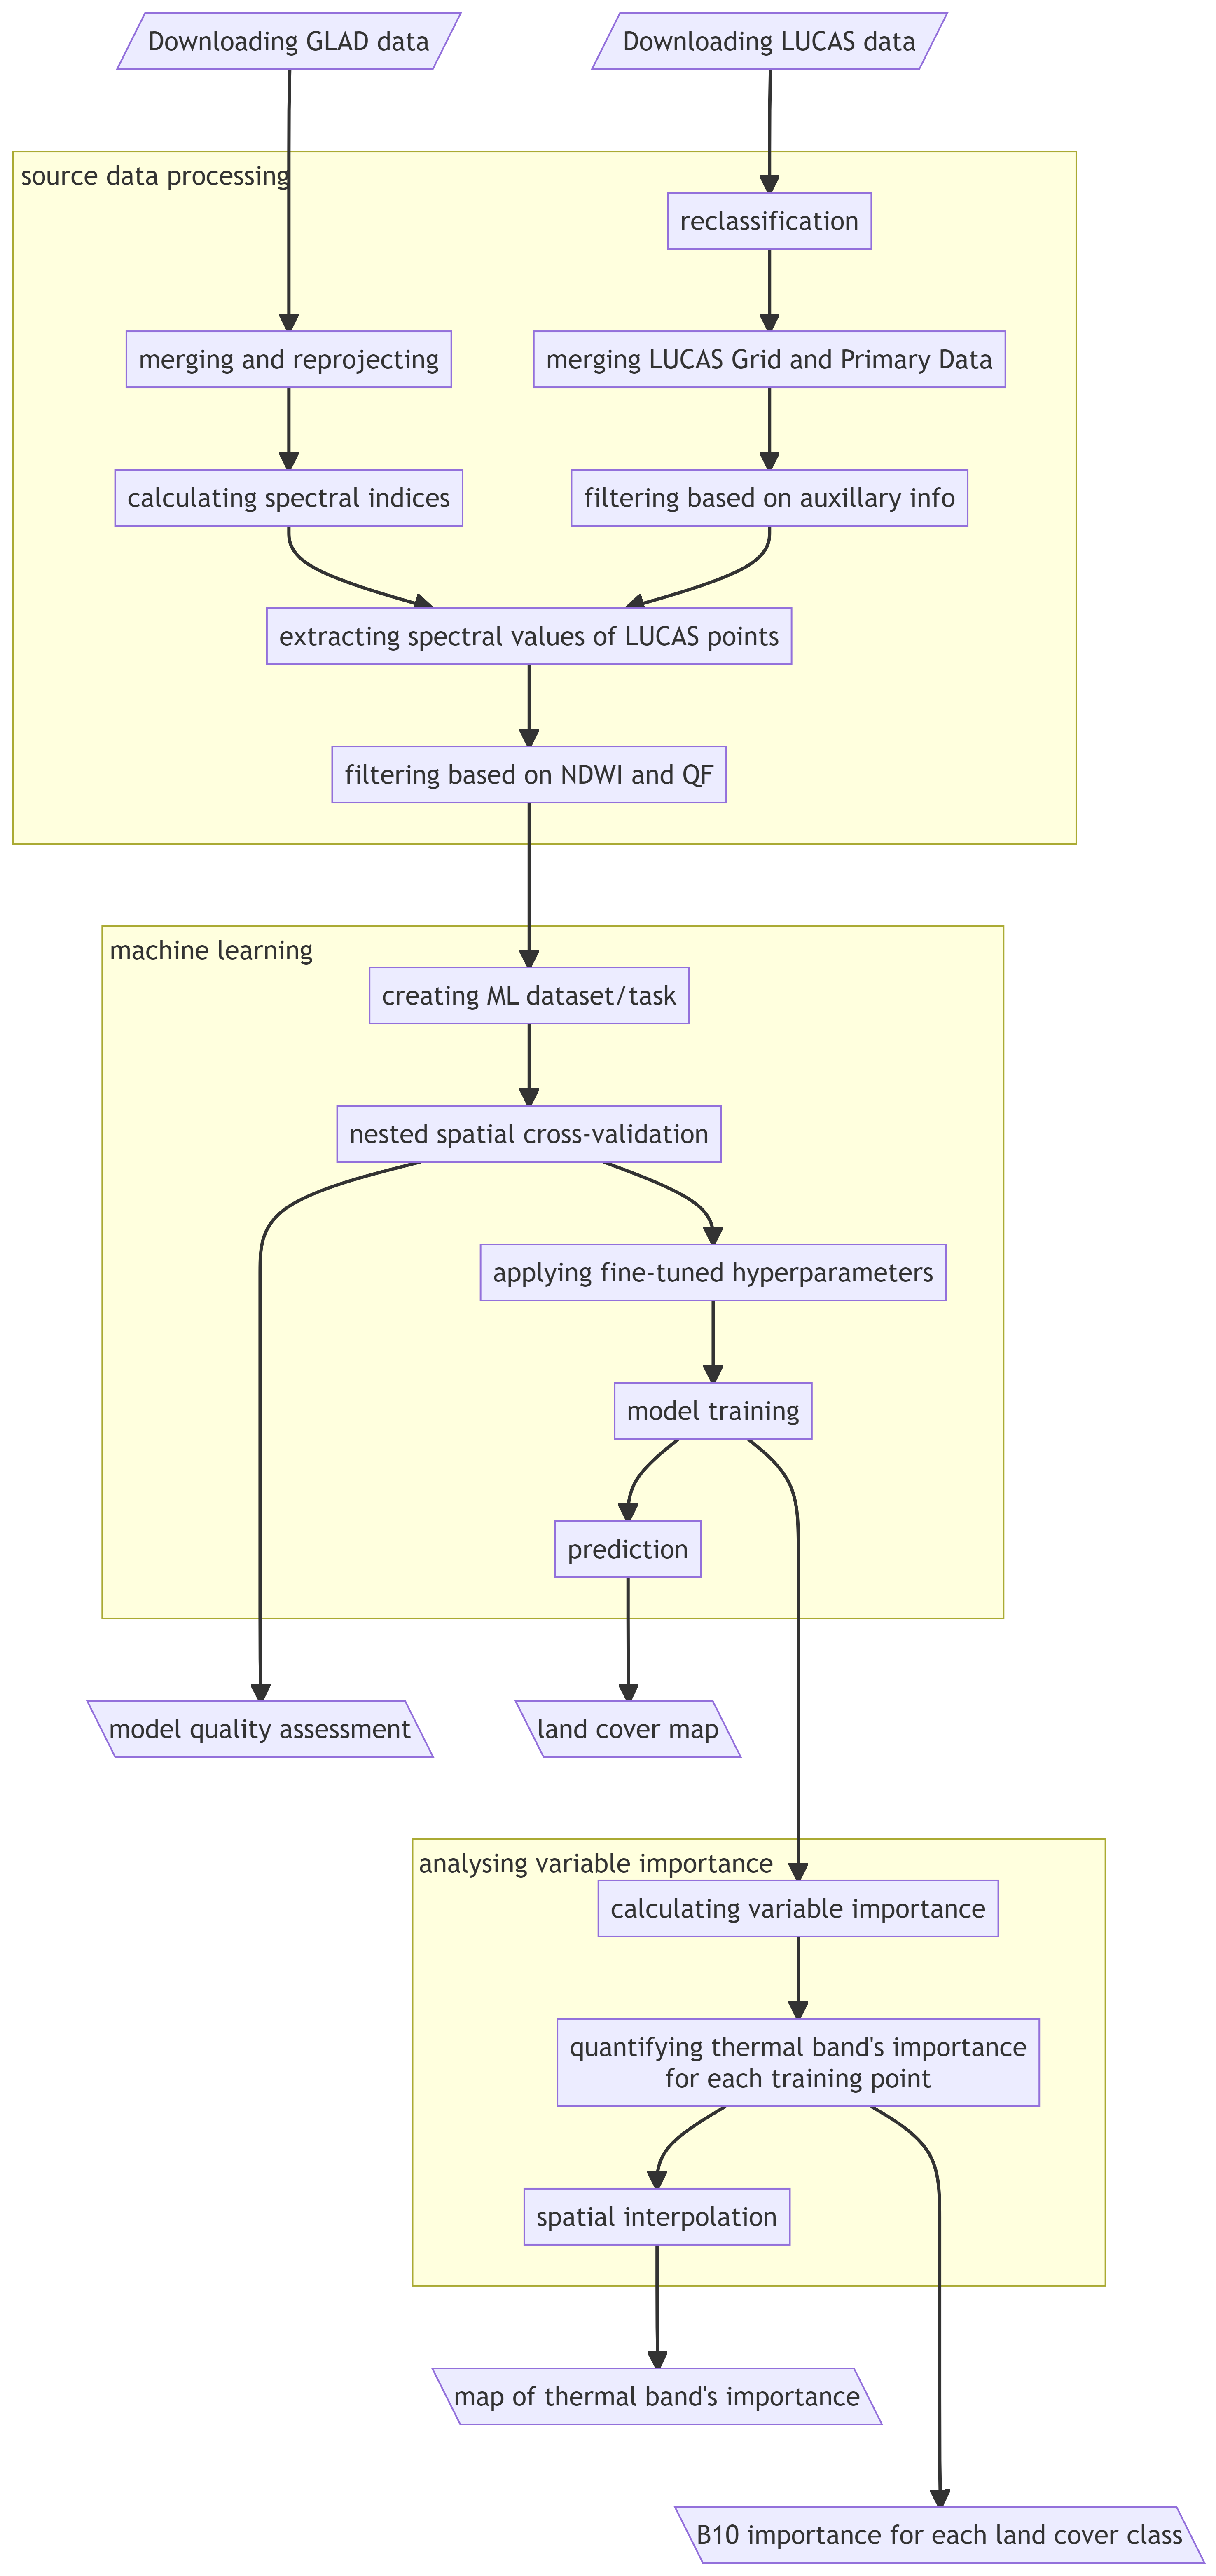
\includegraphics[width=4in,height=8.28in]{./02-roz2_files/figure-latex/mermaid-figure-1.png}

}

\end{figure}

}

\caption{\label{fig-rycina1}General workflow of the study}

\end{figure}

Landsat ARD dataset, provided by GLAD laboratory at the Univeristy of
Maryland, was used as a source of multi-spectral satellite imagery
\autocite{potapov_landsat_2020}. Training points were obtained from
LUCAS dataset created by Eurostat \autocite{dandrimont_harmonised_2020}.
Both datasets were downloaded for central-western part of Poland which
was chosen as the training area (Figure~\ref{fig-rycina2}). This data
was preprocessed and then used to train the model and validate its
performance.

\begin{figure}[H]

{\centering 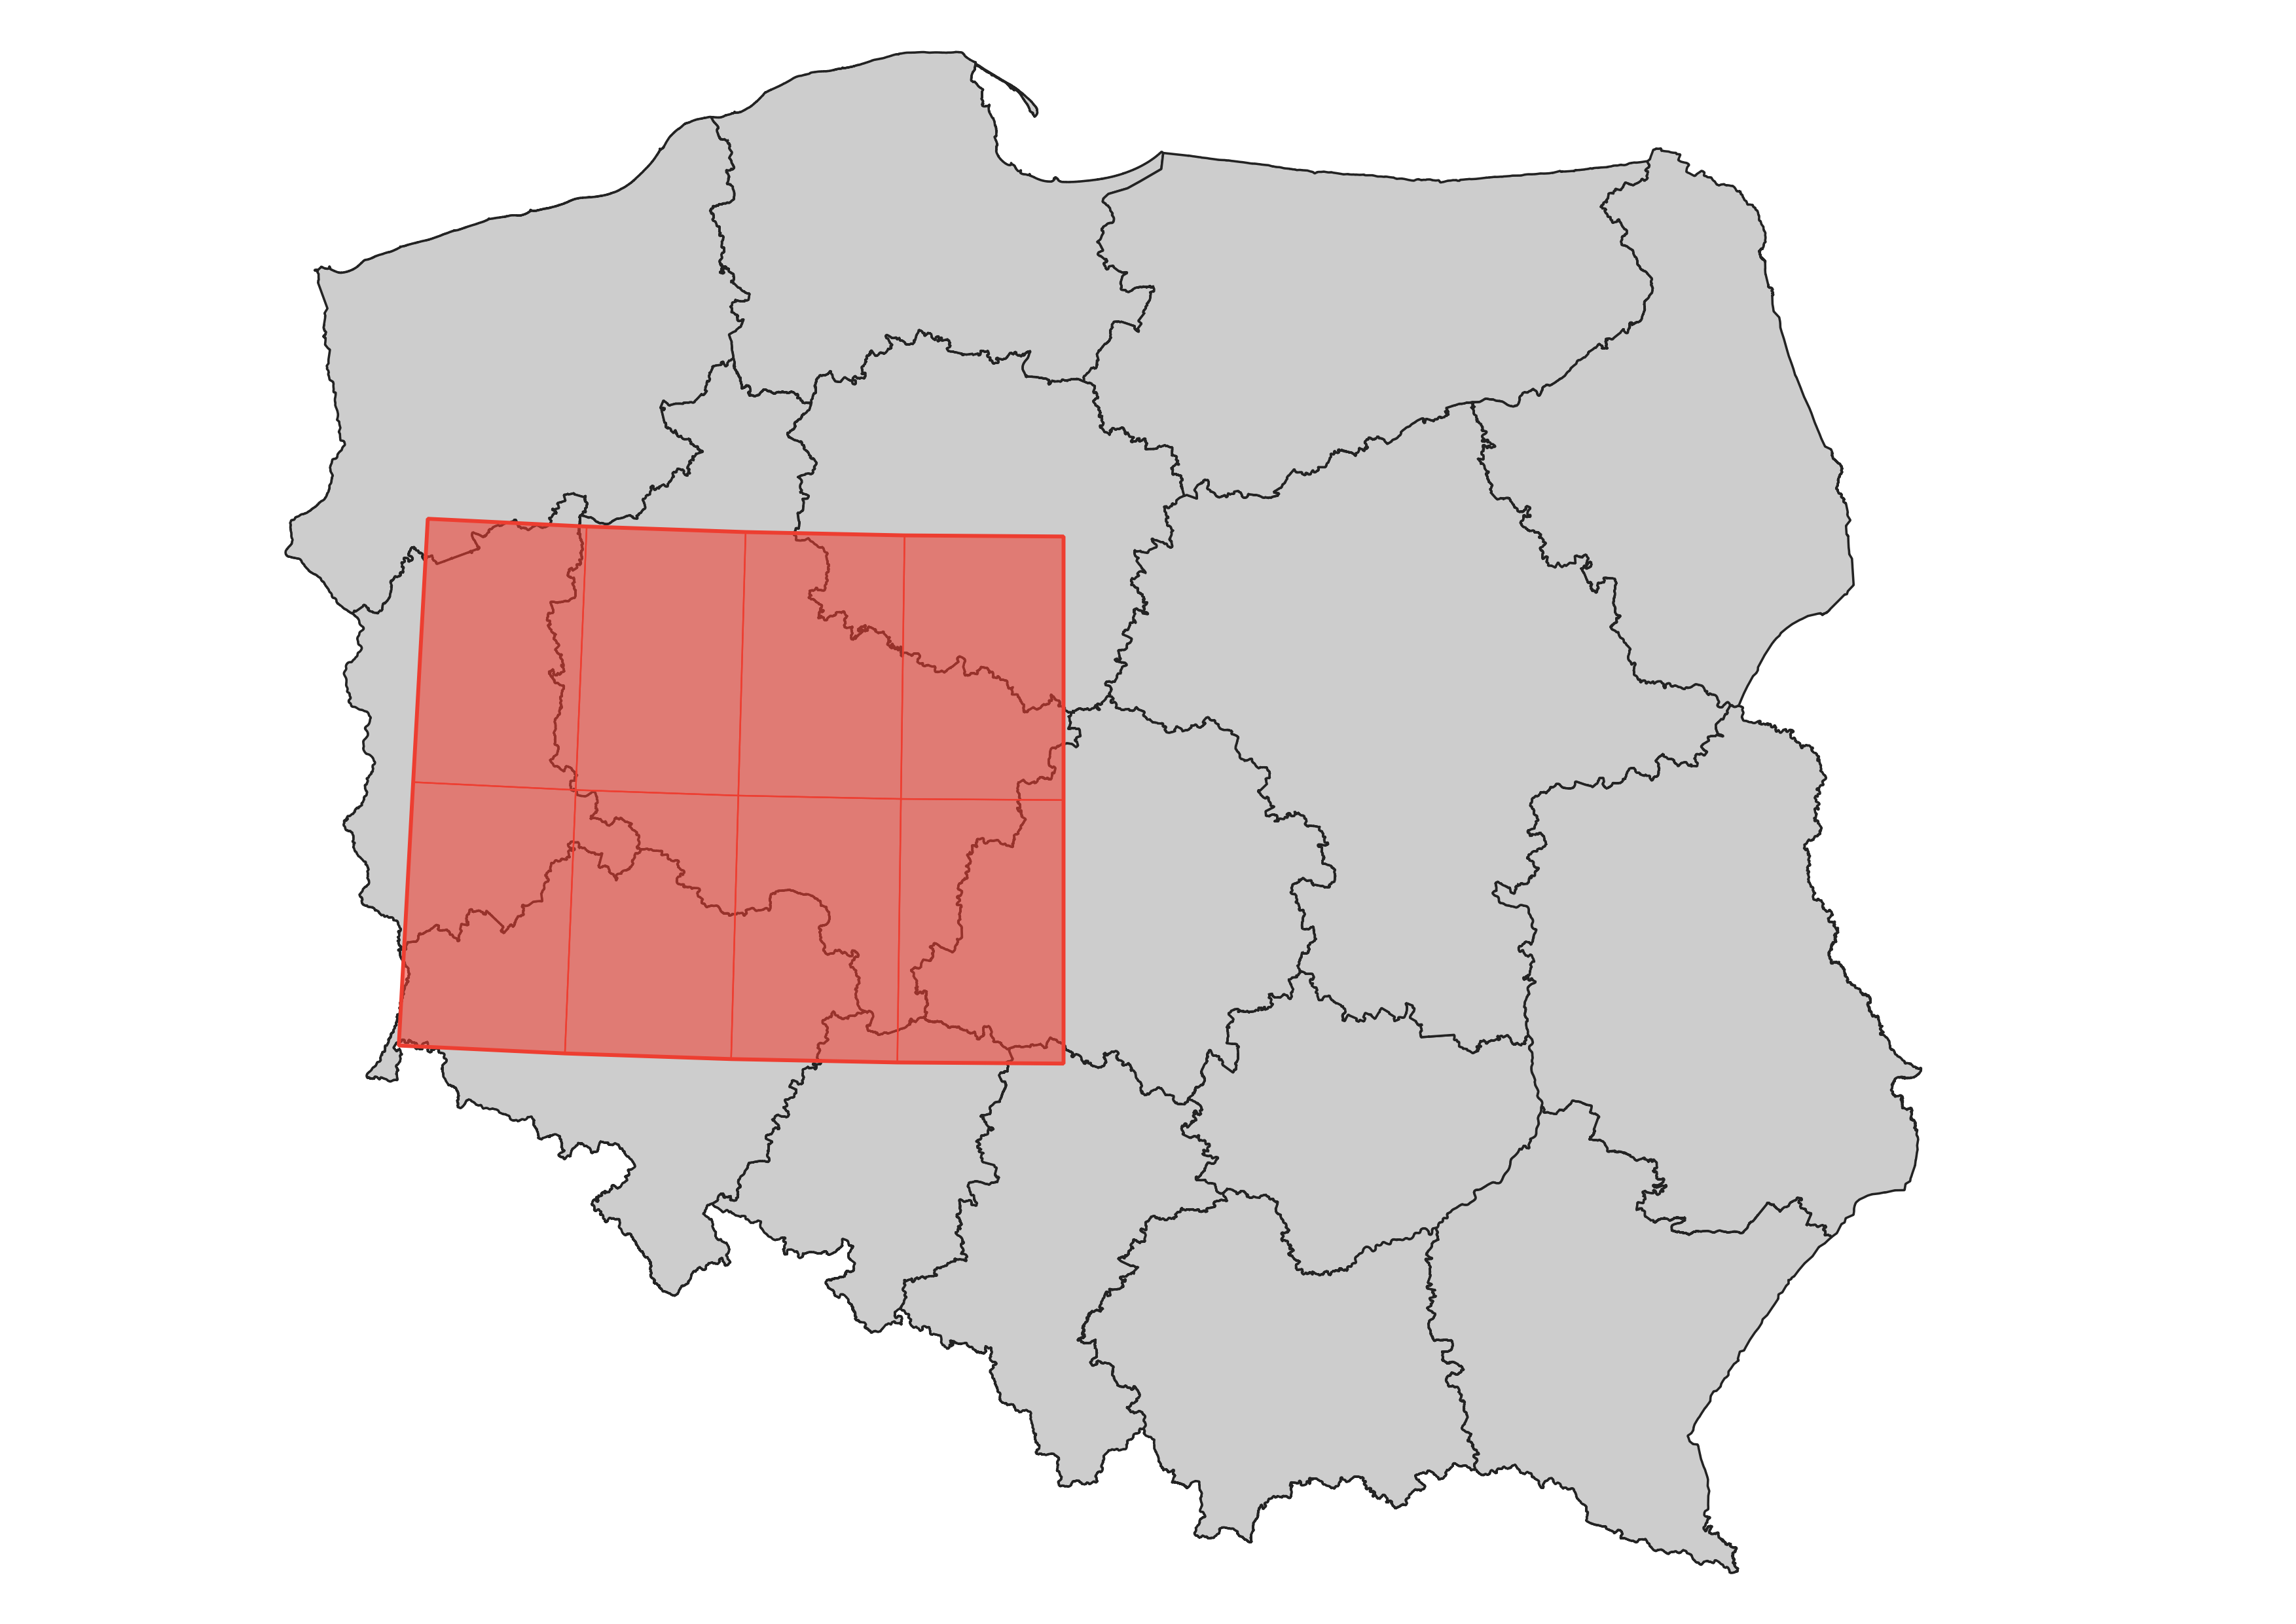
\includegraphics[width=5.875in,height=4.16667in]{./figures/study_area.png}

}

\caption{\label{fig-rycina2}Area covered by the downloaded satellite
imagery}

\end{figure}

\hypertarget{sec-sat}{%
\section{Satellite imagery}\label{sec-sat}}

Satellite imagery from GLAD Landsat ARD product is available in 16-day
interval composites and is divided into 1° x 1° tiles. Processing of
original Landsat images performed by the GLAD team included converting
spectral bands' information to top-of-atmosphere (TOA) reflectance,
converting thermal band values to brightness temperature (BT) in
Kelvins, scaling the values of all bands, as well as, adding quality
flag (QF) for every pixel \autocite{potapov_landsat_2020}.

Satellite images for eight 1° x 1° tiles, covering the study area, were
downloaded using GLAD Tools v1.1 and PERL programming language
(Figure~\ref{fig-rycina1}). These images are from 10th interval of the
year 2018, so downloaded mosaics consist of images acquired between
24.05.2018 and 8.06.2018. All downloaded images were merged and
reprojected from the WGS 84 coordinate reference system (EPSG:4326) to
UTM zone 33N (EPSG:32633). Every band was also resampled from its
original 0.00025° resolution (corresponding to 27.83 m on the equator)
to 30 meters.

In addition, four spectral indices were derived: Normalized Difference
Vegetation Index \autocite[NDVI:][]{tucker_red_1979}, Modified
Normalized Difference Water Index
\autocite[MNDWI:][]{xu_modification_2006}, Normalized Difference
Moisture Index \autocite[NDMI:][]{jin_comparison_2005} and Modified Bare
soil Index \autocite[MBI:][]{nguyen_modified_2021}. Formulas used to
calculate these indices can be found in Table~\ref{tbl-tabela1}.

\hypertarget{tbl-tabela1}{}
\begin{table}
\caption{\label{tbl-tabela1}Formulas of spectral indices derived from Landsat data }\tabularnewline

\centering
\begin{tabular}{|>{\raggedright\arraybackslash}p{4cm}|>{}l|>{}l|}
\toprule
\textbf{band/index} & \textbf{abbreviation} & \textbf{formula}\\
\midrule
Blue & B2 & -\\
\hline
Green & B3 & -\\
\hline
Red & B4 & -\\
\hline
Near Infrared & B5 (NIR) & -\\
\hline
Short-wave Infrared 1 & B6 (SWIR1) & -\\
\hline
Short-wave Infrared 2 & B7 (SWIR2) & -\\
\hline
Thermal & B10 (TIRS1) & -\\
\hline
Normalized Difference Vegetation Index & NDVI & (B5 -B4) / (B4 + B5)\\
\hline
Modified Normalized Difference Water Index & MNDWI & (B3 - B6) / (B3 + B6)\\
\hline
Normalized Difference Moisture Index & NDMI & (B5 - B6) / (B5 + B6)\\
\hline
Modified Bare Soil Index & MBI & (B6 - B7 - B5) / (B6 + B7 + B5) + 0.5\\
\bottomrule
\end{tabular}
\end{table}

\hypertarget{sec-landcover}{%
\section{Land cover data}\label{sec-landcover}}

Data collected during the LUCAS field survey performed by Eurostat was
chosen as a land cover training set. At the moment of writing, it is the
most accurate and comprehensive dataset containing information about
land use and land cover \autocite{pflugmacher_mapping_2019} due to the
fact that every point was either manually photo-interpreted or assessed
during an \emph{in-situ} visit.

LUCAS field survey consists of two phases. The first phase is based on a
grid of points with 2 km spacing covering whole territory of the
European Union (which equals to more than 1 million points). Each point
of the grid is visually interpreted using ortho-photos or satellite
images, and classified into one of seven major land-cover classes. These
classes are: arable land, permanent crops, grassland, wooded areas/shrub
land, bare land, artificial land and water
\autocite{oliver_buck_analysis_2015}. In the second phase, a subsample
of grid points is selected and then visited by Eurostat surveyors. They
classify each point according to full LUCAS land cover and land use
classification. The survey takes place in the spring and summer in order
to observe chosen places in their high vegetation season
\autocite{dandrimont_harmonised_2020}.

Surveyors not only assign land cover and land use classes to points, but
they also add auxillary information such as plant species present at the
site, percentage of land coverage of a chosen class, height of the trees
and their maturity, as well as information about local water management
and irrigation. If there are more than one land cover/land use types at
the point, observer can also assign a secondary class for every LUCAS
point \autocite{oliver_buck_analysis_2015}.

The majority of the training points used in the classification model
were from the second phase of LUCAS survey, also called LUCAS Primary
Data. I downloaded a total of 4,153 points for the study area. The
pre-processing step included omitting records with missing data,
excluding artificial linear land cover classes (e.g.~roads or railways)
and excluding points that were surveyed more than 500 meters from their
theoretical location. In the next step, detailed land cover classes were
aggregated into eight main groups of land cover types. Two of them -
grassland and shrubland were additionally aggregated into one land cover
class due to their spectral and descriptive similarity. Then, I filtered
some of the points according to the percentage of land cover class
coverage or percentage of impervious surface coverage
(Table~\ref{tbl-tabela2}). This step reduced number of unreliable
training points with mixed land cover, e.g.~points with assigned class
covering less than 50\% of surface around it.

\hypertarget{tbl-tabela2}{}
\begin{table}
\caption{\label{tbl-tabela2}Filters applied to reclassified land cover groups. IMP - impervious
surface, HRB - herbaceous plants cover, TC - tree cover }\tabularnewline

\centering
\begin{tabular}{|>{}l|>{}l|>{}l|>{\raggedright\arraybackslash}p{4cm}|>{\raggedright\arraybackslash}p{2cm}|}
\toprule
\textbf{ID} & \textbf{LC class} & \textbf{LUCAS Grid} & \textbf{LUCAS Primary Data} & \textbf{Filters}\\
\midrule
\cellcolor[HTML]{e8ef5f}{\textbf{1}} & arable land & - & B00 (Cropland) & <30\% IMP\\
\hline
\cellcolor[HTML]{80dc59}{\textbf{2}} & grassland & - & E00 (Grassland), D00 (Shrubland) & >50\% HRB; <30\% IMP\\
\hline
\cellcolor[HTML]{11a723}{\textbf{3}} & forests & - & C00 (Woodland) & >50\% TC; <20\% IMP\\
\hline
\cellcolor[HTML]{b7b7b7}{\textbf{4}} & bare land & 6 (Bare surface) & F00 (Bare land) & -\\
\hline
\cellcolor[HTML]{ea001f}{\textbf{5}} & artificial land & 7 (Artificial areas) & A00 (Artificial land) & >70\% IMP\\
\hline
\cellcolor[HTML]{56a4f3}{\textbf{6}} & water bodies & 8 (Inland water) & G00 (Water areas) & -\\
\hline
\cellcolor[HTML]{7a338c}{\textbf{7}} & wetlands & - & H00 (Wetlands) & -\\
\bottomrule
\end{tabular}
\end{table}

For the least frequent classes in the LUCAS Primary Data dataset - bare
land, artificial land and water bodies - I also added points classified
during the first phase of LUCAS survey (Figure~\ref{fig-rycina3}). This
step was necessary to ensure that every land cover class is represented
by enough points. It was not possible only for the wetlands class,
because of the lack of such category in the first phase classification.
At the end of the pre-processing, dataset had 3,778 training points.

\begin{figure}[H]

{\centering 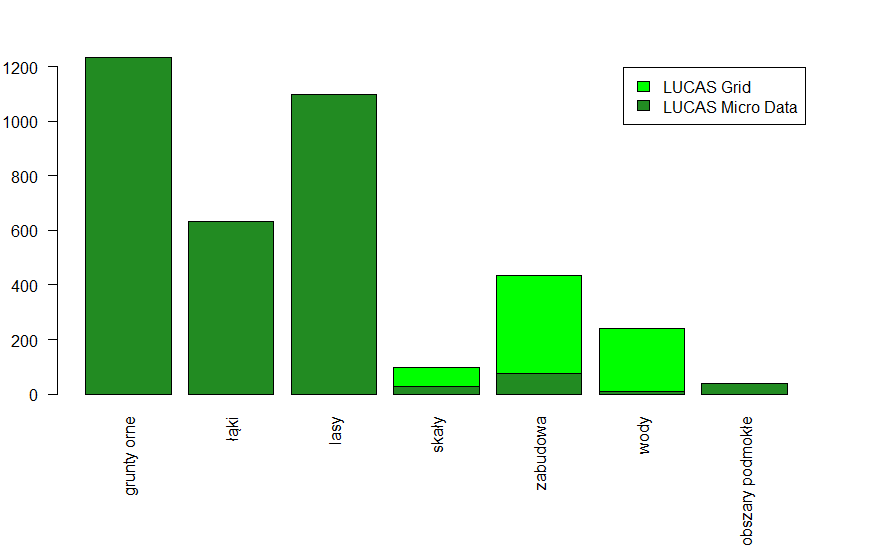
\includegraphics[width=5.79167in,height=3.64583in]{./figures/lucas_data.png}

}

\caption{\label{fig-rycina3}Distribution of points by land cover class
after pre-processing}

\end{figure}

After extracting values from Landsat ARD raster, LUCAS points were also
filtered using the quality flag provided. Only points with the clear-sky
quality flag were taken into account during the model training.
Moreover, water bodies points in which NDWI was lower than 0 were also
excluded. These two conditions eliminated 404 points in total.

The training set obtained after pre-processing can be seen in
Figure~\ref{fig-rycina4}. Spatial distribution of data points was fairly
even and due to the structure of LUCAS data set, every point was located
2 kilometers or further from the next one.

\begin{figure}[H]

{\centering 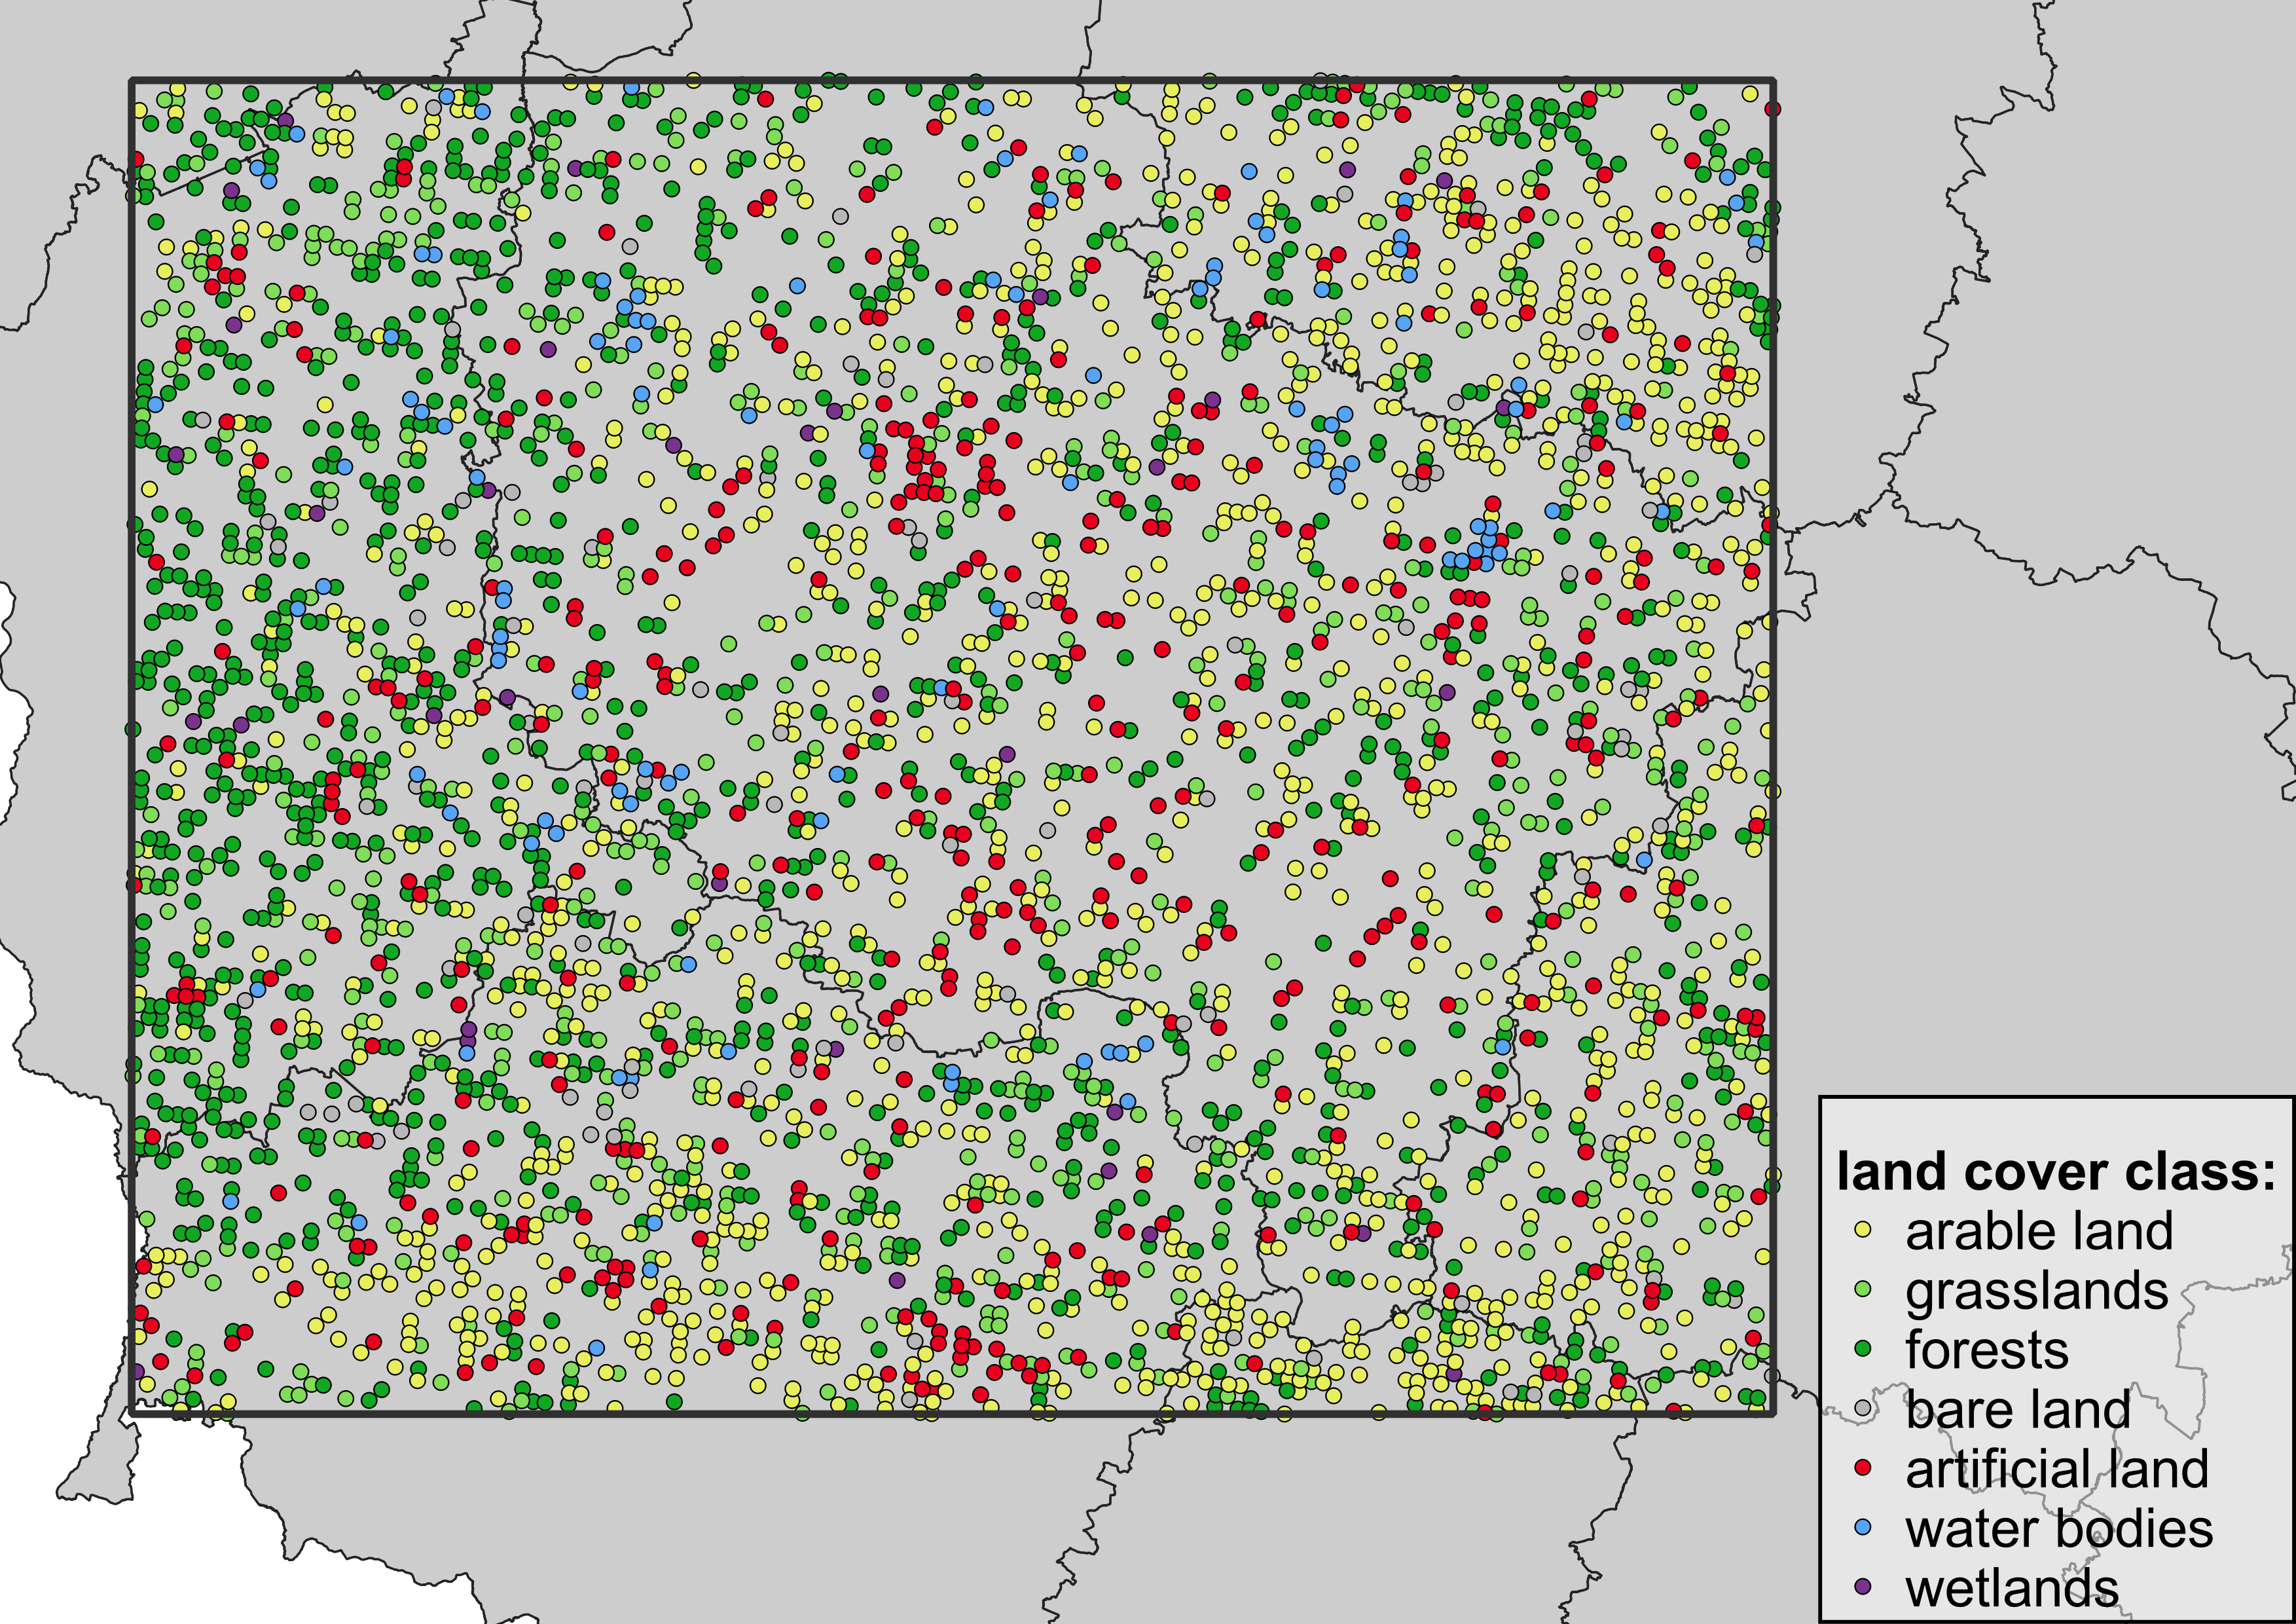
\includegraphics[width=5.875in,height=4.16667in]{./figures/lucas_distribution.png}

}

\caption{\label{fig-rycina4}Spatial distribution of LUCAS training
points after pre-processing}

\end{figure}

\hypertarget{sec-ml}{%
\section{Machine learning}\label{sec-ml}}

Machine learning is a computation method used to teach machines from
datasets automatically, without being specifically programmed
\autocite{mahesh_machine_2018,sarker_machine_2021}. We can divide
machine learning methods into two main groups: supervised and
unsupervised.

Unsupervised learning analyzes unlabeled datasets without the need for
human intervention. This is widely used for extracting generative
features, identifying meaningful trends and structures, grouping results
and for exploratory purposes \autocite{sarker_machine_2021}. This type
of machine learning discovers hidden patterns or data groupings
(clusters) which is used in exploration analysis or objects
segmentation.

Supervised learning uses labeled training data and a collection of
training examples, which are used by an algorithm to find relationships
between different variables. It is carried out when certain goals are
identified to be accomplished from a certain set of inputs. There are
two main types of supervised learning tasks: classification (separating
data) and regression (fitting data) \autocite{sarker_machine_2021}.

In this study, supervised classification algorithm called Random Forest
(RF) was used \autocite{breiman_random_2001}.

\hypertarget{sec-rf}{%
\subsection{Random forest algorithm}\label{sec-rf}}

I chose Random Forest as an algorithm used in this study, since it is
considered to be the best classification algorithm for land cover
mapping \autocite{talukdar_land-use_2020}. It is a very popular machine
learning tool thanks to its high interpretability and relatively high
accuracy \autocite{qi_random_2012}. Other advantages of this algorithm
is its ability to handle missing values, wide spectrum of accepted
variable types (continuous, binary, categorical) and ease of modelling
high-dimensional data \autocite{qi_random_2012}. Random Forest consists
of a specified number of decision trees, which are based on series of
splitting rules.

A decision tree aims to partition the dataset into smaller, more
homogeneous groups \autocite{kuhn_applied_2013}. This process creates a
set of rules by dividing dataset into several categories. Each rule in
the decision tree is specified by a feature (variable used to split) and
a threshold (value of a feature dividing dataset)
\autocite{sekulic_random_2020}. Random Forest algorithm is characterized
by using many decision trees at the same time and receiving results by
applying majority voting system based on outputs of all decision trees
\autocite{kuhn_applied_2013}. Each tree in the forest has slightly
different input data - a subset of data is sampled with replacement to
get different result in every tree. This process is known as bagging or
bootstrap aggregating \autocite{schonlau_random_2020}. Moreover,
algorithm is allowed to use only a subset (randomly sampled) of
available variables in every split which reduces correlation between
trees \autocite{sohil_introduction_2022}.

\newpage

\hypertarget{sec-resampling}{%
\subsection{Model quality assessment and
fine-tuning}\label{sec-resampling}}

Accuracy of the model was assessed using five performance measures:

\begin{itemize}
\item
  Overall accuracy: ratio of number of correct predictions to the total
  number of input points
\item
  Kappa coefficient: how well the classification performed as compared
  to assigning values randomly
\item
  Recall (producer's accuracy): how often are real features on the
  ground correctly shown on the classified map
\item
  Precision (user's accuracy): how often the class on the map will
  actually be present on the ground
\item
  F1-score: harmonic mean between precision and recall, measures if
  classifier both classifies data correctly and does not miss a
  significant number of points
\end{itemize}

Every above metric, except Kappa coefficient, takes values from 0 to 1.
Value of 0 means poor model performance and value of 1 means high
quality of the model. As for Kappa coefficient, its values range from -1
to 1. Values below 0 mean worse agreement between data distributions
than random chance and values above 0 (up to 1) mean model performing
better than random.

Values of these indices were estimated with the help of resampling
technique called spatial cross-validation (CV)
\autocite{lovelace_geocomputation_2019}. It is a type of
cross-validation that divides dataset into folds and also considers
spatial aspect of the data.

In \emph{k}-fold cross-validation, every data point is used in both
training and testing set. Whole dataset is randomly divided into
\emph{k} equal parts (\emph{folds}). Then, machine learning model is
independently trained \emph{k} times and in each run, different part of
the dataset is used as validation set, while remaining \emph{k - 1}
parts are used to fit the model. This way, every data point is used in
the testing set only once and is used to train the model in the
remaining runs \autocite{jiao_performance_2016}. Usually, whole
cross-validation procedure is repeated several times to get higher
number of unique dataset splits and to receive more reliable average
values of the overall accuracy \autocite{varga_validation_2021}. Such
approach is a compromise which enables possibility of using a whole
dataset in the training process of the final model without a need of
acquiring independent testing set in order to measure model's
performance.

Since this study is based on geographic data, spatial autocorrelation
needs to be taken into account. As Tobler stated: ``Everything is
related to everything else, but near things are more related than
distant things'' \autocite{tobler_computer_1970}. In order to prevent
testing points from being related to training points, I applied spatial
cross-validation approach which aims to prevent the model to overfit to
the training data. This method is different than regular
cross-validation only in the partitioning step - instead of randomly
dividing dataset into groups, location of data points is used together
with k-means clustering \autocite{brenning_spatial_2012} in order to
create spatially disjoint folds \autocite{lovelace_geocomputation_2019}.
Thanks to this partitioning method, spatial bias can be significantly
reduced which leads to more reliable performance estimation. Example of
such approach can be seen in Figure~\ref{fig-rycina5}.

\begin{figure}[H]

{\centering 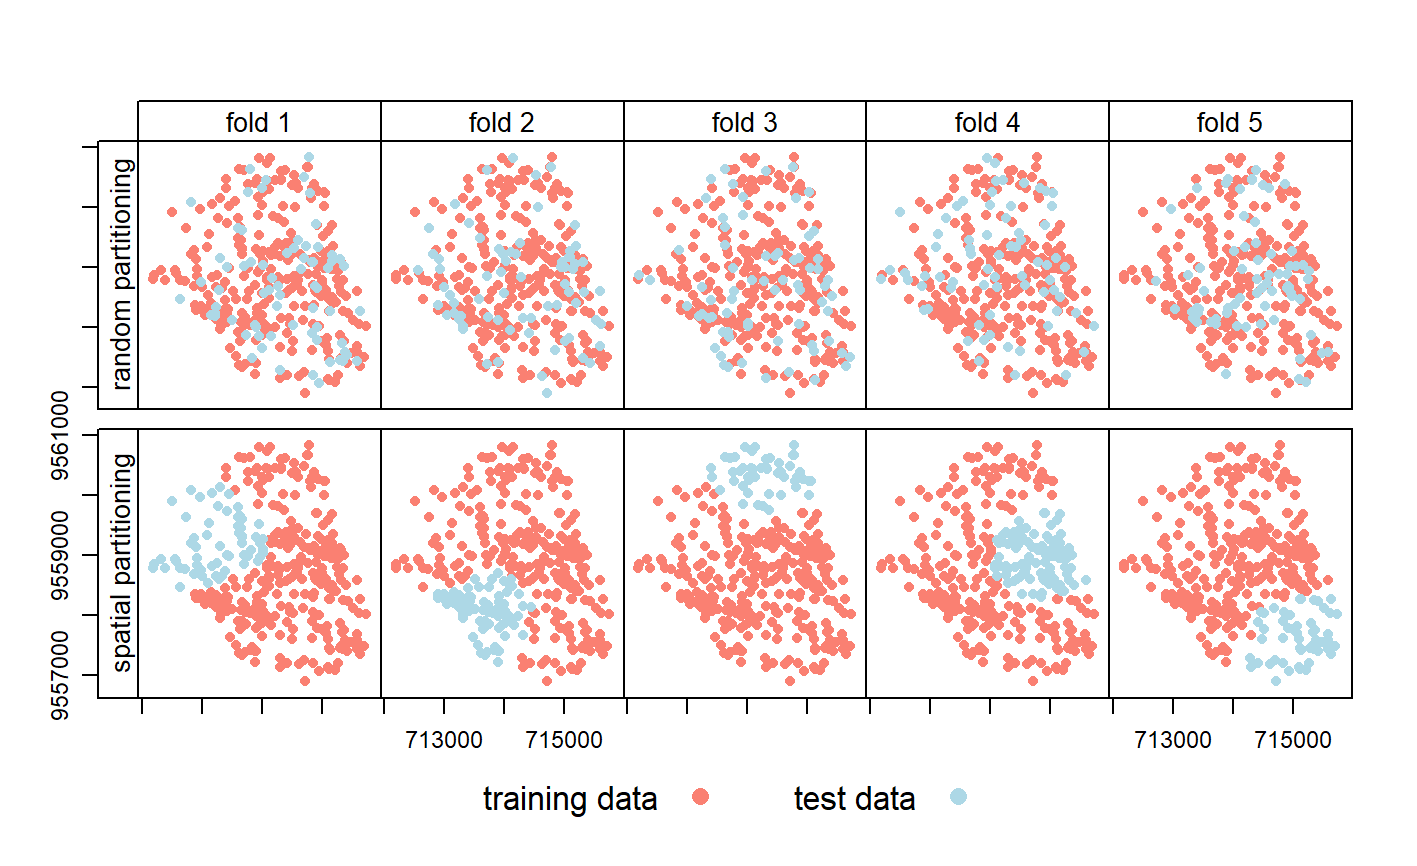
\includegraphics[width=5.9375in,height=3.64583in]{./figures/spatial_partitioning.png}

}

\caption{\label{fig-rycina5}Comparison of random and spatial
partitioning of dataset for cross-validation on external example data
\autocite[Source:][]{lovelace_geocomputation_2019}}

\end{figure}

Random Forest algorithm takes several hyperparameters as an input in
order to specify how much should it fit to training data. Optimizing
these parameters is crucial for tree-based machine learning models
\autocite{yang_hyperparameter_2020}. Model's hyperparameters can be
fine-tuned to find values that give the best model accuracy.

With the aim to determine values of model's hyperparameters as
accurately as possible, I performed nested spatial cross-validation.
This method is an extension of previously described approach, with
hyperparameter tuning added to the process. Each fold created in the
spatial CV is further divided into next \emph{n} folds which comprise
the tuning level of the process. Then, another \emph{n}-fold
cross-validation is performed on these folds in order to determine
performance of randomly sampled hyperparameter values. The best
hyperparameter combination is chosen to train the model on outer fold
(performance estimation level) \autocite{schratz_hyperparameter_2019}.
Whole process is then repeated on every of \emph{k} outer folds which
leads to the most accurate performance measurement as well as defining
the best hyperparameter setting.

I chose three hyper-parameters for tuning: number of trees, maximum
depth of the tree and minimal size of each node in decision tree. I used
overall accuracy achieved by each classifier to rank their performance
and choose parameters that train the model best. On the tuning level of
every fold in spatial CV process, I examined 10 random configurations of
hyperparameters and assessed their performance by applying 5-fold inner
resampling. Parameters' search spaces and tuning result received from
nested cross-validation can be found in Table~\ref{tbl-tabela3}.

\hypertarget{tbl-tabela3}{}
\begin{table}
\caption{\label{tbl-tabela3}Hyperparameters of RF model optimized during nested spatial
cross-validation }\tabularnewline

\centering
\begin{tabular}{|>{}l|>{}l|>{}l|}
\toprule
\textbf{Hyper-parameter} & \textbf{Search space} & \textbf{Optimal value}\\
\midrule
number of trees & 50 - 500 & 186\\
\hline
maximum depth & 5 - 100 & 99\\
\hline
min. node size & 1 - 50 & 2\\
\bottomrule
\end{tabular}
\end{table}

\newpage

\hypertarget{sec-importance}{%
\section{Variable importance and its spatial
distribution}\label{sec-importance}}

Quantifying importance of model's variables is a part of evaluating its
results. It can be used for model simplification and exploration,
domain-knowledge-based validation or knowledge generation
\autocite{biecek_explanatory_2021}. This study was focused on the latter
purpose since its aim was to check if thermal information has a
significant impact on land cover classification.

Importance of model variables can be measured on two levels: dataset
level and instance level \autocite{biecek_explanatory_2021}. On the
dataset level, we can measure change in model accuracy depending on the
presence of one chosen variable (Section~\ref{sec-importance-dataset}).
This gives basic knowledge about this variable's impact on model
predictions. Assessing importance on the instance (observation) level
helps to understand an impact of variables for one specific data point
(Section~\ref{sec-importance-instance}). Moreover, the instance level
importance can be utilized to interpolate variable importance values
from points into continuous raster data
(Section~\ref{sec-importance-distribution}).

\hypertarget{sec-importance-dataset}{%
\subsection{Dataset level}\label{sec-importance-dataset}}

Measuring variable importance on the dataset level requires evaluating
model twice: once with original data and once with permuted values of
the considered variable. The main idea behind this action is to measure
difference between models' performance. Breiman
\autocite*{breiman_random_2001} assumes that if a variable is important,
then model's performance is expected to lower after permuting this
variable's values. For this purpose, cross entropy was used as a loss
function thus its change was considered as a measure of variable
importance \autocite{biecek_explanatory_2021}. In order to measure each
variable's importance, twelve seperate models were created: one with
original data and eleven modified models, each one with different
variable's values permuted. Comparison of these eleven models and the
original model made possible quantifying impact of every variable on the
original model results. This value is treated as an overall variable
importance on the dataset level.

There is also a visual method to explore variable importance on dataset
level. It is based on interpreting partial-dependence (PD) profiles of
variables (Figure~\ref{fig-rycina6}). Such plot shows how does
probability of choosing certain class changes as a function of the
selected variable \autocite{biecek_explanatory_2021}. Values for PD
profile are calculated by averaging Ceteris-paribus profiles created for
every observation in the dataset. This approach is an easy and intuitive
way to understand variables' impact on model results. If probability
values of choosing certain class do not change along with the changes of
variable's value, we can assume that this variable does not have big
impact on model predictions or that our model did not detect such
dependence.

\begin{figure}[H]

{\centering 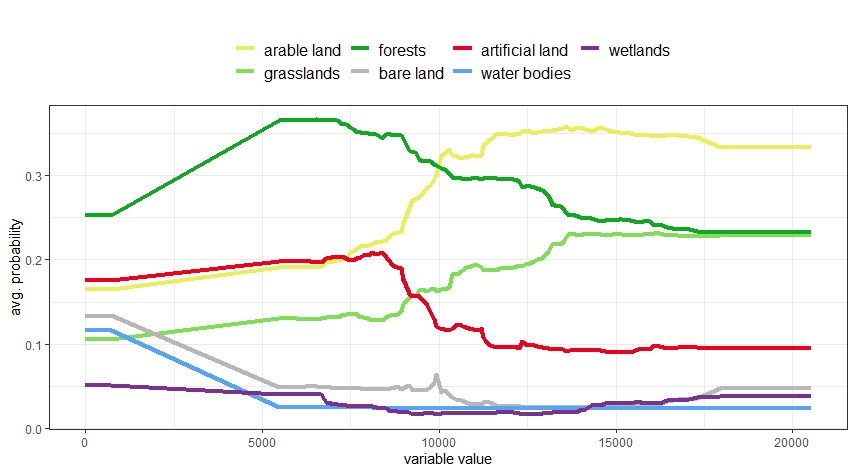
\includegraphics[width=5.625in,height=3.125in]{./figures/profB5.png}

}

\caption{\label{fig-rycina6}Example partial-dependence profile for
near-infrared band (B5)}

\end{figure}

\hypertarget{sec-importance-instance}{%
\subsection{Instance level}\label{sec-importance-instance}}

Another way to measure variable importance in machine learning models is
the instance level evaluation. It helps to find out how much each
variable contributed to the model's outcome for a particular observation
\autocite{biecek_explanatory_2021}. One way of calculating variable
impact on the observation result is creating a break-down plot
(Figure~\ref{fig-rycina7}). Its main idea is to estimate contribution of
variable by measuring the change in model predictions while fixing the
values of consecutive variables to values recorded for the chosen
observation \autocite{biecek_explanatory_2021}. After fixing the value
of variable for whole dataset, change in model prediction is calculated.
This value indicates the variable impact on a chosen observation.

\begin{figure}[H]

{\centering 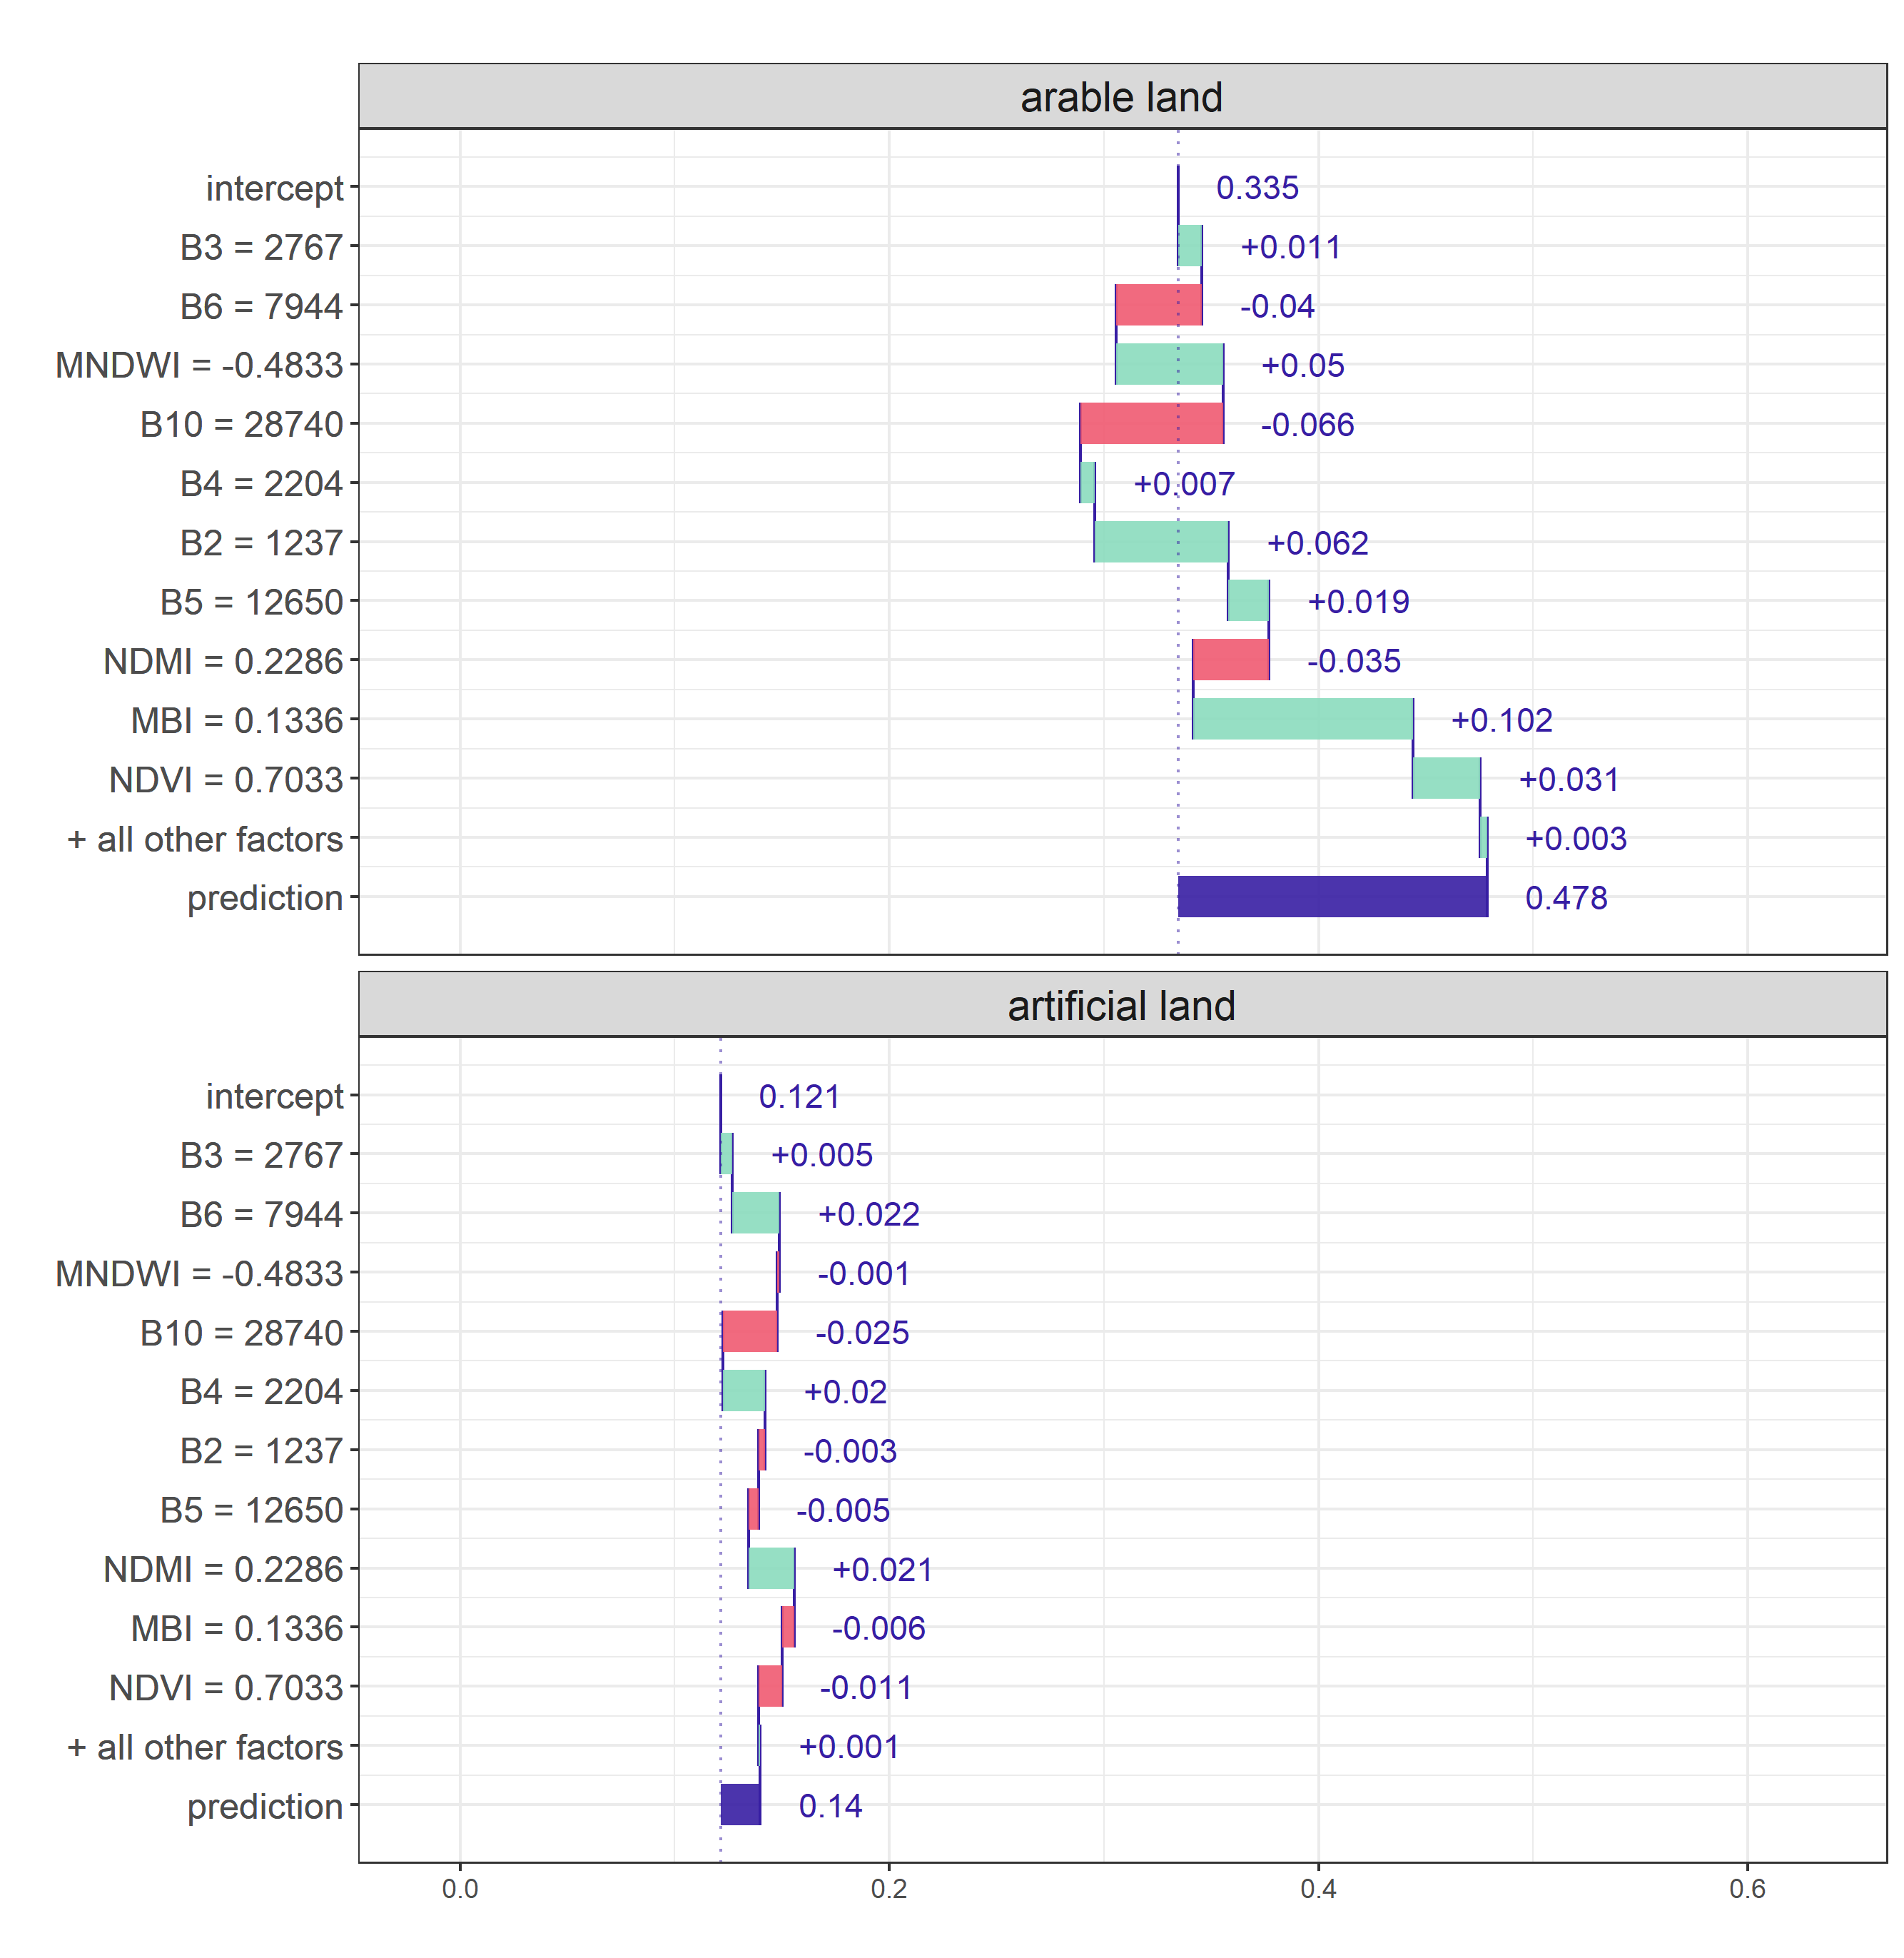
\includegraphics[width=4.54167in,height=4.6875in]{./figures/break-down_plot.png}

}

\caption{\label{fig-rycina7}Example of a break-down plot that visualises
variables' impact on chosen observation}

\end{figure}

However, above method is highly dependent on variable ordering and
interactions between these variables \autocite{biecek_explanatory_2021}.
To address this issue, I applied another approach based on averaging
values from multiple break-down plots, each one with different ordering
of the variables. This method originates from ``Shapley values''
\autocite{shapley_value_1953} and was adapted to machine learning by
Štrumbelj and Kononenko \autocite*{strumbelj_efficient_2010}. Main idea
of this approach is to apply several different variable orderings,
create a break-down plot for each of them and calculate the mean value
of contribution for each variable (Figure~\ref{fig-rycina8}). Thanks to
this method, the influence of variable ordering can be mostly removed
\autocite{biecek_explanatory_2021}.

\begin{figure}[H]

{\centering 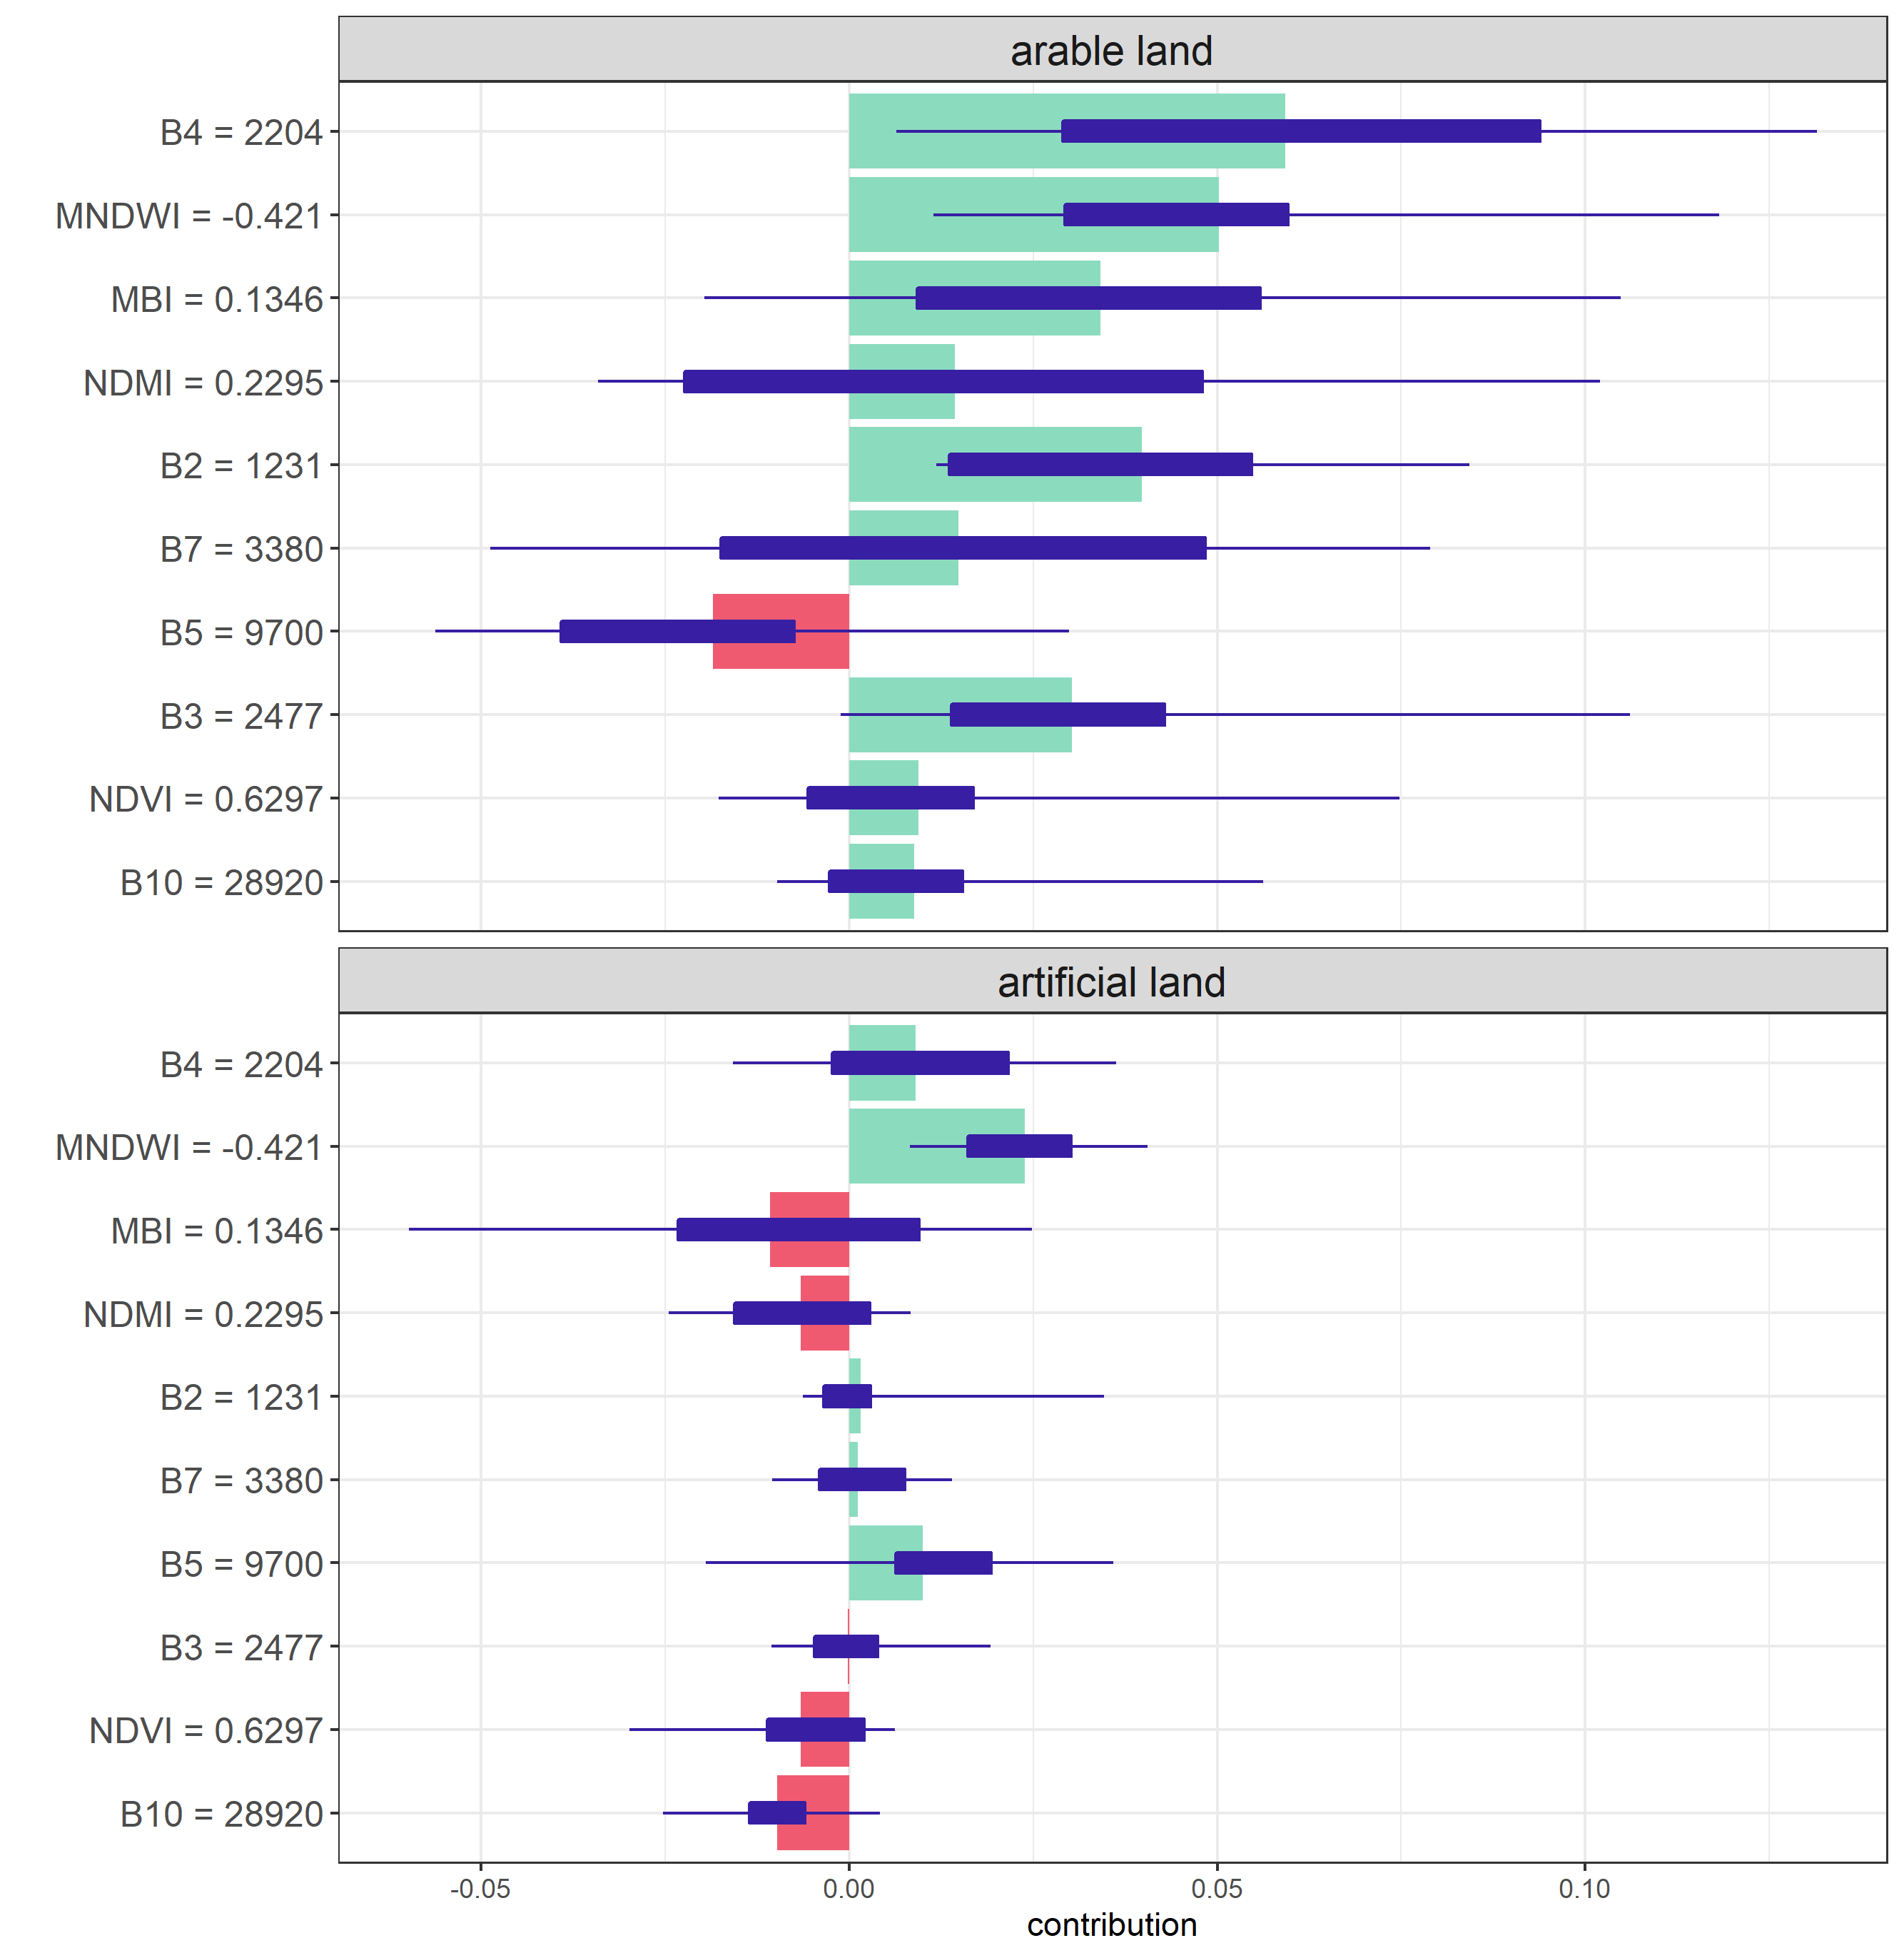
\includegraphics[width=4.54167in,height=4.6875in]{./figures/shapley_values.png}

}

\caption{\label{fig-rycina8}Example plot of Shapley Additive
Explanations. Green and red bars show average variable contribution to
model result. Blue box plots show distribution of variable contributions
across different variable orderings.}

\end{figure}

Eventually, Shapley values provide a possibilty to measure contribution
of each variable in every observation in the training set. Such result
enables us to add spatial context to the variable importance, which is
further described in Section \ref{sec-importance-distribution}.

\hypertarget{sec-importance-distribution}{%
\subsection{Spatial distribution}\label{sec-importance-distribution}}

In order to estimate spatial distribution of variable importance values,
I applied two different approaches. First of them is based on the raster
aggregation - resampling of satellite imagery from 30 m to 1.5 km
resolution. Lowering the resolution of the data and averaging band
values highly decreases computational time, as well as helps to discover
more general trends and patterns rather than local ones. After
resampling, Shapley values were calculated for every raster cell and
variable importance was measured.

The second approach utilizes LUCAS training points used during a model
training together with spatial interpolation techniques. First, Shapley
values are calculated for every point and importance of variable is
assigned to them. This step is followed by spatial interpolation of
variable importance values from points to continuous raster layer with
the help of the Inverse Distance Weighting (IDW) interpolation method.

Both approaches have their pros and cons. Raster aggregation method is
spatially more consistent, but averaging of spectral values may not
entirely represent objects on the ground. On the other hand, point
interpolation method is very accurate for places near LUCAS points
location, but values for more distant areas may not be as reliable.

\hypertarget{sec-r}{%
\section{R language environment}\label{sec-r}}

Almost every step of analysis described in previous sections was
performed with the use of R \autocite{R-base} - an open-source
programming language designed mainly for statistical computing and
visualizing data. I used RStudio \autocite{rstudio_team_rstudio_2020} as
an integrated development environment (IDE). Apart from base R
functionalities, a number of packages created by the R community were
implemented into workflow. I used \emph{terra} package
\autocite{R-terra} to perform raster data operations and \emph{sf}
\autocite{R-sf} to manipulate and process vector data. To conduct
machine learning steps of the analysis, I used an environment of various
machine learning packages called \emph{mlr3} \autocite{R-mlr3}. Random
forest algorithm used by \emph{mlr3} framework is part of the
\emph{ranger} package \autocite{R-ranger}. I also used \emph{dplyr}
\autocite{R-dplyr} and \emph{tidyr} packages \autocite{R-tidyr} to clean
and process tabular data. \emph{DALEX} \autocite{R-DALEX} and
\emph{DALEXtra} \autocite{R-DALEXtra} packages provided various
functionalities enabling me to estimate variable importance and
visualize these results with the help of the \emph{ggplot2} package
\autocite{R-ggplot2}. Moreover, the \emph{corrplot} package was used to
calculate and visualize correlation matrix of Landsat data in order to
explore dataset in more detail. Package called \emph{gstat}
\autocite{R-gstat} helped to interpolate variable importance values from
points to a continuous raster layer. In addition, the \emph{future}
package \autocite{R-future} was used to enable multi-threading of some
computationally intensive tasks.

\bookmarksetup{startatroot}

\hypertarget{sec-results-map}{%
\chapter{Land cover map}\label{sec-results-map}}

The main product of the model is a land cover map of Poznań metropolitan
area (Figure~\ref{fig-rycina9}). Moreover, the created model contains
probabilities of choosing each class for every pixel of the raster
layer. With the help of this information, a probability map showing
model's confidence in its choice of land cover class was created
(Figure~\ref{fig-rycina11}). Value of each pixel reflects the highest
probability assigned to one of seven land cover classes.

After a visual analysis of Figure~\ref{fig-rycina9}, some conclusions
about its general accuracy can be made. Overall distributions of main
land cover classes such as urban areas (artificial land), forests,
arable land and water bodies, seem to be correctly recognized.

\begin{figure}[H]

{\centering 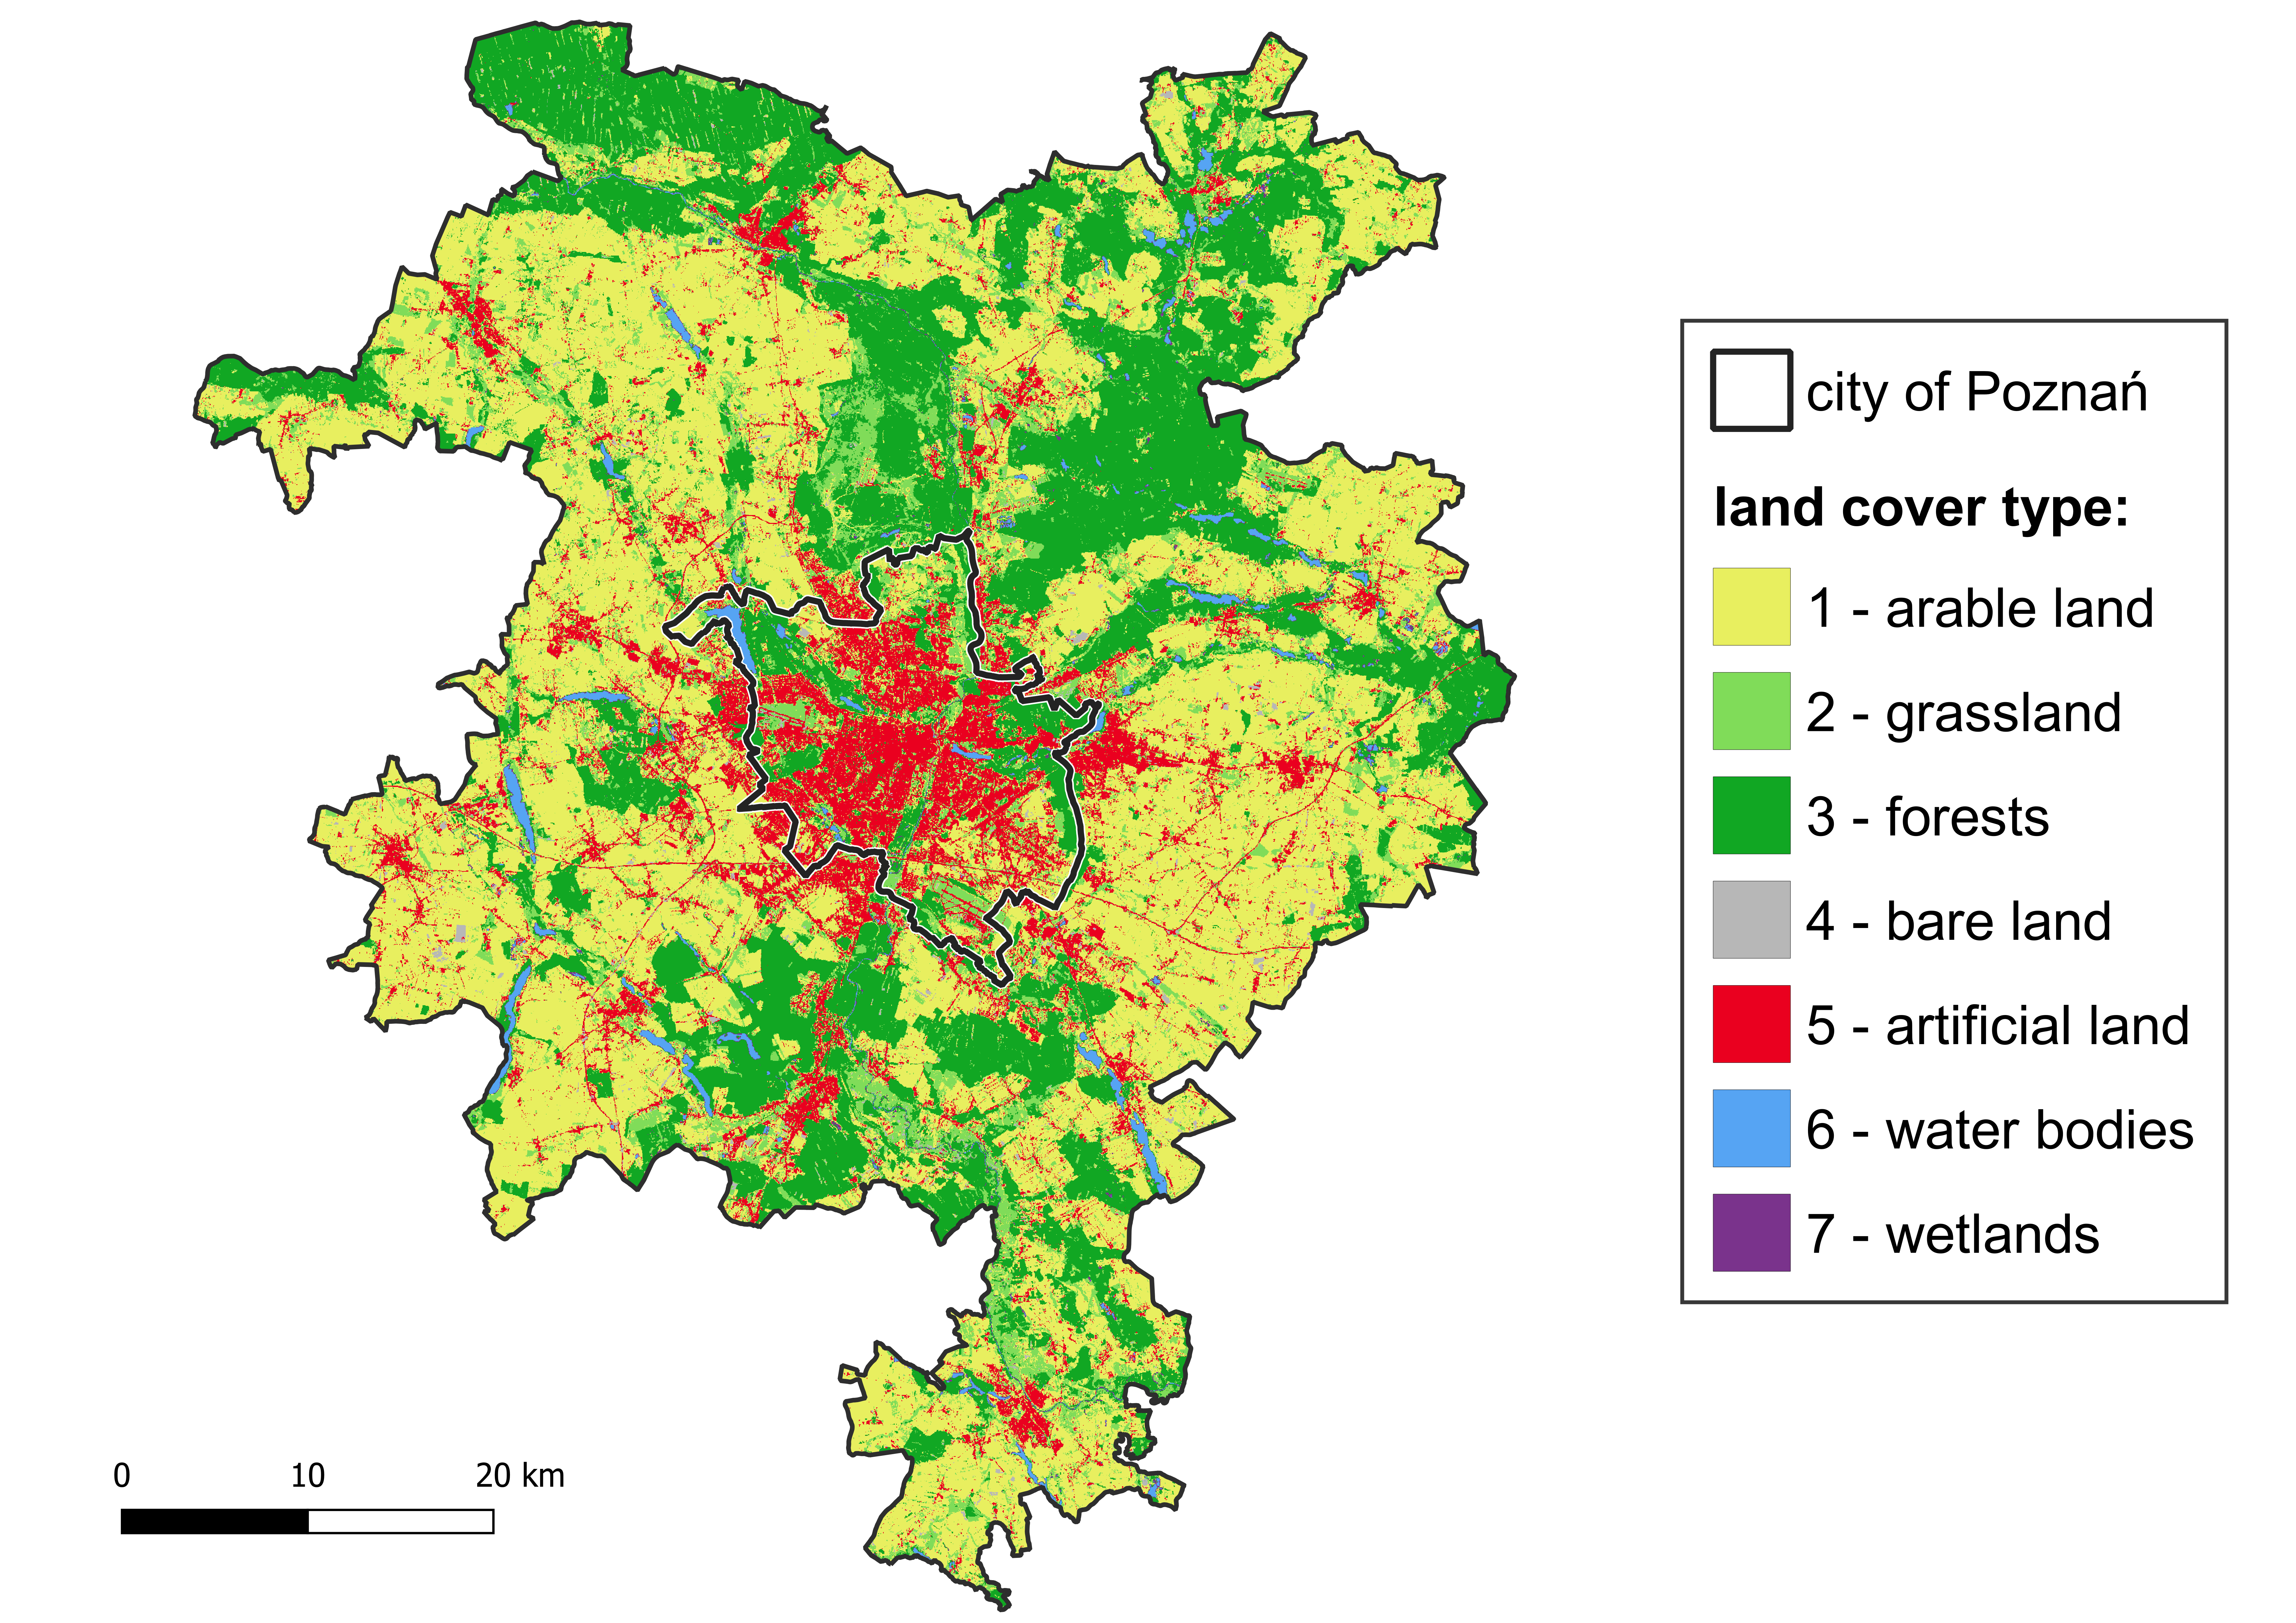
\includegraphics[width=5.875in,height=4.16667in]{./figures/result_map-lc.png}

}

\caption{\label{fig-rycina9}Land cover map of Poznań metropolitan area
created during this study}

\end{figure}

In order to investigate model's predictive accuracy on a local scale,
six arbitrary chosen sites were examined more closely
(Figure~\ref{fig-rycina10}). Locations of sites were selected to present
different landscape patterns on the studied map, as well as point out
some common mistakes made by the model. Visual analysis of these sites
showed that the model correctly recognizes most of land cover patterns
present on the ground. At the same time, there were several bigger
problems and mistakes in its predictions. For instance, there are many
examples of single pixels in the artificial area being classified as
arable land (especially in sites 1, 2 and 6). Urban areas on the created
map are generally more fragmented than they are in reality. Moreover,
some cropland areas were incorrectly classified as grassland (sites 4, 5
and 6). Another problem occurred in the classification of a river
surface - its shape on the land cover map was not continuous and water
was often misclassified as wetland (sites 1 and 5). On the other hand,
the model has managed to correctly recognize wetlands in sites 2 and 4,
despite the fact that no training point of wetlands class was located
nearby.

\begin{figure}[H]

{\centering \includegraphics[width=5.20833in,height=9.0625in]{./figures/comparison.png}

}

\caption{\label{fig-rycina10}Comparison of the created land cover map
(b) with GLAD satellite imagery (a) and ortophotomap from Polish
Geoportal (c)}

\end{figure}

Analysis of the model's confidence derived from the probability map
(Figure~\ref{fig-rycina11}) showed visible spatial autocorrelation. In
order to derive mean values of confidence for every land cover class,
zonal statistics were calculated. Highest values of confidence were
recorded for forests (0.86) and water bodies (0.92). For urban areas and
arable land, model's confidence was lower at mean level of 0.64 and
0.71, respectively. The model was least confident in recognizing bare
land (0.44), wetlands (0.46) and grassland (0.57).

\begin{figure}[H]

{\centering \includegraphics[width=5.875in,height=4.16667in]{./figures/result-map-prob.png}

}

\caption{\label{fig-rycina11}Probability of a chosen land cover class
being present on the ground. This can be treated as a confidence of the
model on its results.}

\end{figure}

\bookmarksetup{startatroot}

\hypertarget{sec-results-eval}{%
\chapter{Assessing model quality}\label{sec-results-eval}}

As mentioned in Section~\ref{sec-resampling}, in order to evaluate model
performance nested \emph{k}-fold spatial cross-validation was performed.
I chose approach with 5 folds and 10 repetitions. Hyperparameter tuning
level of nested resampling used 5 folds to evaluate 10 different
hyperparameter combinations. This resulted in total of 2500 models
created both for performance estimation and hyperparameter tuning.
Results of these models were then evaluated and quality measures were
computed. In Table~\ref{tbl-tabela4}, overall quality measures, such as,
accuracy and Kappa coefficient are presented. Moreover, I calculated
weighted precision, recall and F1-score. Weights for these calculations
were based on number of observations from each land cover class.
Original precision, recall and F1-score values by land cover type are
shown in Table~\ref{tbl-tabela5}.

In general, model achieved accuracy level of 0.752 with the Kappa
coefficient of 0.652. These values are rather average and model indeed
needs some improvements. On the other hand, this performance is enough
to assess thermal band's importance (Chapter~\ref{sec-results-therm}),
which is the main goal of this study.

\hypertarget{tbl-tabela4}{}
\begin{table}
\caption{\label{tbl-tabela4}Overall performance measures calculated during
cross-validation/resampling process }\tabularnewline

\centering
\begin{tabular}{|>{}l|>{}r|}
\toprule
\textbf{Measure} & \textbf{Average value}\\
\midrule
overall accuracy & 0.752\\
\hline
Kappa coefficient & 0.652\\
\hline
precision (user's accuracy) & 0.742\\
\hline
recall (producer's accuracy) & 0.751\\
\hline
weighted F1-score & 0.743\\
\bottomrule
\end{tabular}
\end{table}

An in-depth analysis of performance measures by land cover class shows
that precision and recall values for certain type are similar
(Table~\ref{tbl-tabela5}). This means that model did not have any
specific problem either with too many false positive (FP) or false
negative (FN) predictions. It was just not that good for some classes.
Model performed very poorly in terms of correctly classifying
observations of wetlands class but it is quite common issue across many
studies (for example, \textcite{malinowski_automated_2020}). Also bare
land class had low values of model quality with F1-score of 0.242. The
main problem concerning these land cover classes is that there was
probably not enough training points for each of them in the study area.
On the other hand, two largest classes in terms of number of
observations - arable land and forests - were classified much more
accurately, with F1-score of 0.777 and 0.889 respectively. Land cover
type with the highest values of precision and recall, despite of low
number of observations, was the water bodies class. Model performed very
good for this class probably because of its distinct spectral
characteristics and easily distinguishable borders.

\hypertarget{tbl-tabela5}{}
\begin{table}
\caption{\label{tbl-tabela5}Performance measures by land cover class }\tabularnewline

\centering
\begin{tabular}{|>{}l|>{}r|>{}r|>{}r|}
\toprule
\textbf{Land cover class} & \textbf{Recall (producer's accuracy)} & \textbf{Precision (user's accuracy)} & \textbf{F1-score}\\
\midrule
arable land & 0.732 & 0.828 & 0.777\\
\hline
grasslands & 0.612 & 0.613 & 0.612\\
\hline
forests & 0.886 & 0.892 & 0.889\\
\hline
bare land & 0.320 & 0.194 & 0.242\\
\hline
artificial land & 0.656 & 0.493 & 0.563\\
\hline
water bodies & 0.971 & 1.000 & 0.985\\
\hline
wetlands & 0.394 & 0.121 & 0.185\\
\bottomrule
\end{tabular}
\end{table}

\bookmarksetup{startatroot}

\hypertarget{sec-results-therm}{%
\chapter{Evaluating thermal band's impact}\label{sec-results-therm}}

As described in Section~\ref{sec-importance}, variable importance can be
assessed both on dataset and instance (observation) level. The latter
was used to estimate spatial distribution of thermal band's importance
in order to present the results on the map.

However, before moving to thermal band's importance assessment, I
explored Landsat dataset more carefully in order to determine correlated
variables and interactions between them. Creating correlation plot
(Figure~\ref{fig-rycina19}) revealed that some bands are highly
correlated - especially these from visible spectrum and SWIR bands. This
may suggest that these variables depend on the other variable's values
\autocite{biecek_explanatory_2021}, thus absence of one variable might
not lower model's performance because other variable can fill this
information gap. On the other hand, feature selection performed with the
help of \emph{mlr3} framework \autocite{R-mlr3} has shown that including
all variables still proves to achieve the best model performance.
Moreover, implemented methods of assessing variable importance
(described in Section~\ref{sec-importance}) are designed to minimize
impact of interactions between variables.

\begin{figure}[H]

{\centering 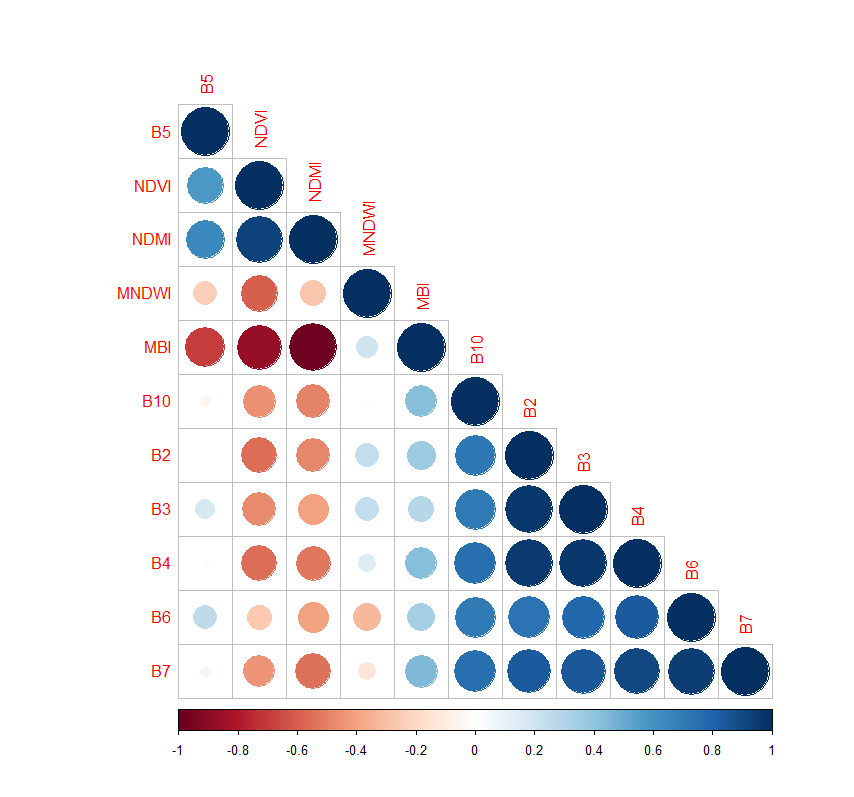
\includegraphics[width=5.57292in,height=5.20833in]{./figures/corrplot.png}

}

\caption{\label{fig-rycina19}Correlation matrix of Landsat bands}

\end{figure}

\hypertarget{sec-imp-overall}{%
\section{Measuring importance of thermal band}\label{sec-imp-overall}}

As a very basic way to check thermal band's importance on model results,
I implemented benchmarking methods with the help of functions provided
by \emph{mlr3} framework \autocite{R-mlr3}. Two datasets (\emph{tasks})
were created: one with thermal band included and one without this
variable. Other hyperparameters of models were the same. Then, 5-fold
spatial cross-validation with 10 repetitions were performed on models
created from both datasets in order to estimate their predictive
abilities. Differences between them were very narrow, but visible -
model with thermal band included achieved higher average accuracy of
approximately 0.4 perc. points and higher average Kappa of approx.
0.006. Moreover, distribution of accuracy values in the boxplot changed
visibly, with higher median accuracy for model with thermal band
included (Figure~\ref{fig-rycina12}). In the end, however, these
differences are rather small and we can not state that thermal band had
strong impact on model predictions.

\begin{figure}[H]

{\centering 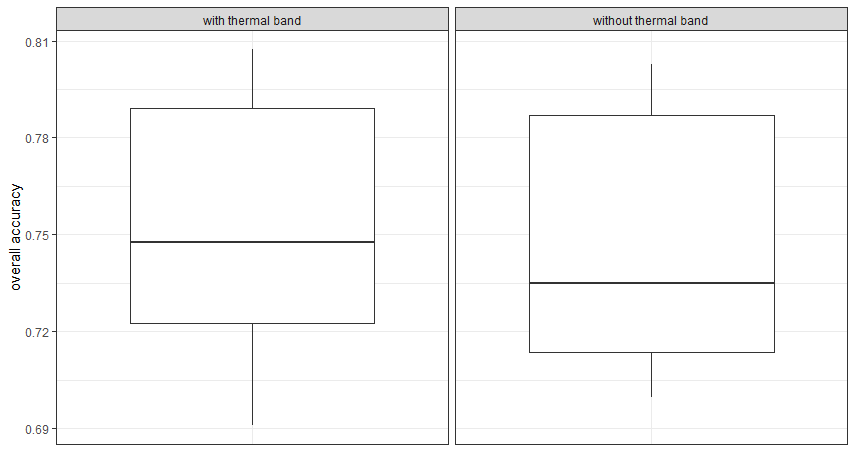
\includegraphics[width=5.625in,height=3.125in]{./figures/model_comparison.png}

}

\caption{\label{fig-rycina12}Accuracy distributions for 50 models with
and without thermal band included}

\end{figure}

In the next step of thermal information importance evaluation, overall
measures were derived. Again, it turned out that thermal band variable
had little impact on the model results. With cross-entropy loss value of
28, it was the least important variable in the dataset. Importance
values of all variables are shown in Figure~\ref{fig-rycina13}.

\begin{figure}[H]

{\centering 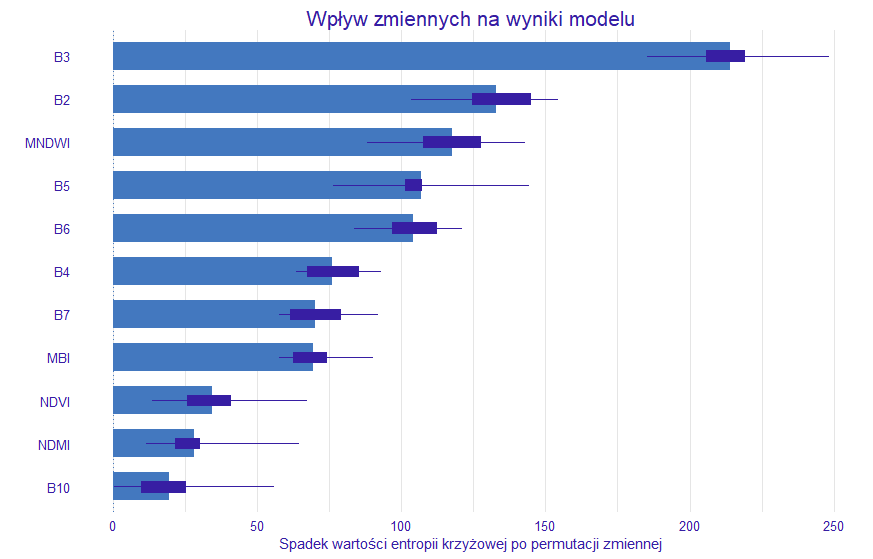
\includegraphics[width=5.625in,height=3.125in]{./figures/importance.png}

}

\caption{\label{fig-rycina13}Overall variable importance expressed as
cross-entropy loss}

\end{figure}

After evaluating variable importance on dataset level, instance level
calculations were performed. Shapley values for each of 166 LUCAS points
in Poznań metropolitan area were computed and thermal band's importance
was derived. This made possible to calculate average thermal band's
importance for each of seven land cover classes. In addition, mean value
of temperature for each class was computed in order to give better
insight into differences between them. Results of these computations are
shown in Table~\ref{tbl-tabela6}. However, it must be emphasized that
166 points was rather small number, especially for less numerous classes
such as wetlands.

Table~\ref{tbl-tabela6} presents differences of thermal band's
importance across land cover types. It was significantly higher for
artificial land and wetlands. Average value for wetlands is not very
reliable though, because there were only 3 such points in studied area -
one of them having much higher value of importance than the other two.
Due to this issue, median value of importance was calculated too. In
this case, value for wetlands was much lower, but median importance
value for artificial areas was nearly the same. Distributions of
importance values can be examined in larger detail in
Figure~\ref{fig-rycina14}.

\hypertarget{tbl-tabela6}{}
\begin{table}
\caption{\label{tbl-tabela6}Mean value and importance of thermal band, by land cover class of LUCAS
points }\tabularnewline

\centering
\begin{tabular}{|>{}l|>{}r|>{}r|>{}r|}
\toprule
\textbf{Land cover class} & \textbf{Mean temp. [°C]} & \textbf{Average importance} & \textbf{Median importance}\\
\midrule
arable land & 20.5 & 0.022 & 0.019\\
\hline
grasslands & 20.5 & 0.020 & 0.016\\
\hline
forests & 16.0 & 0.022 & 0.019\\
\hline
bare land & 21.1 & 0.019 & 0.019\\
\hline
artificial land & 21.9 & 0.046 & 0.046\\
\hline
water bodies & 13.8 & 0.008 & 0.008\\
\hline
wetlands & 15.0 & 0.049 & 0.016\\
\bottomrule
\end{tabular}
\end{table}

\begin{figure}[H]

{\centering 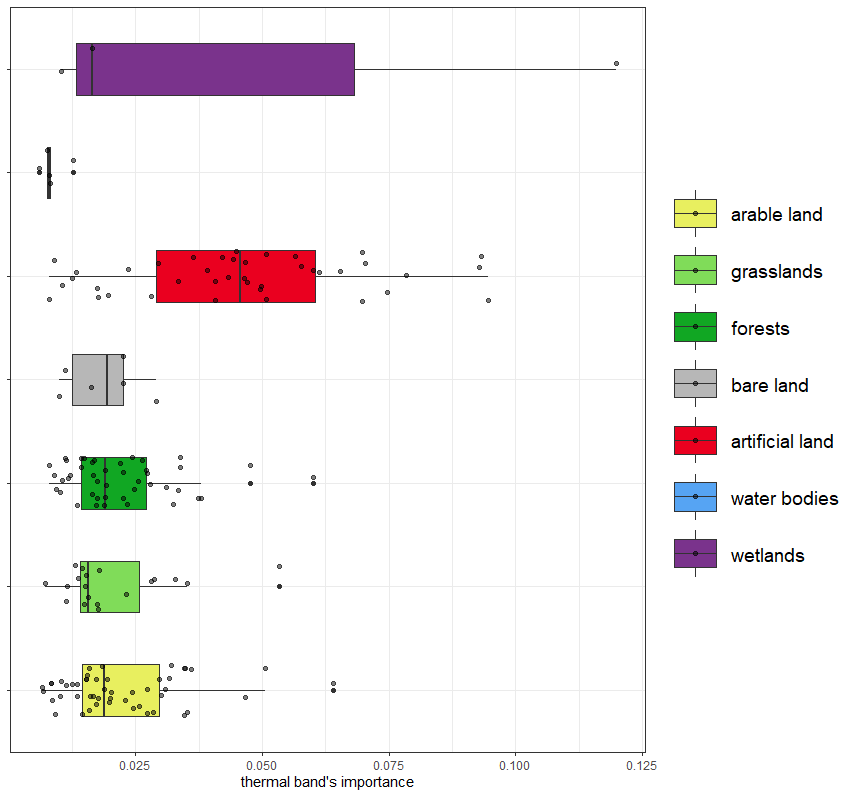
\includegraphics[width=5.05208in,height=5.20833in]{./figures/importance_classes.png}

}

\caption{\label{fig-rycina14}Distributions of thermal band's importance
by land cover class. Small dots show exact values of each LUCAS point.}

\end{figure}

In addition, mean importance values for every land cover class are shown
in Figure~\ref{fig-rycina14a}. With the help of this chart, some
comparisons between land cover classes and variables can be made.
Thermal band's importance for prediction of artificial land turns out
not to be the highest among other variables. Some bands have higher
influence on predicting this land cover type. On the other hand, thermal
band is one of five bands, whose impact for predicting artificial land
was higher than the average.

\begin{figure}[H]

{\centering 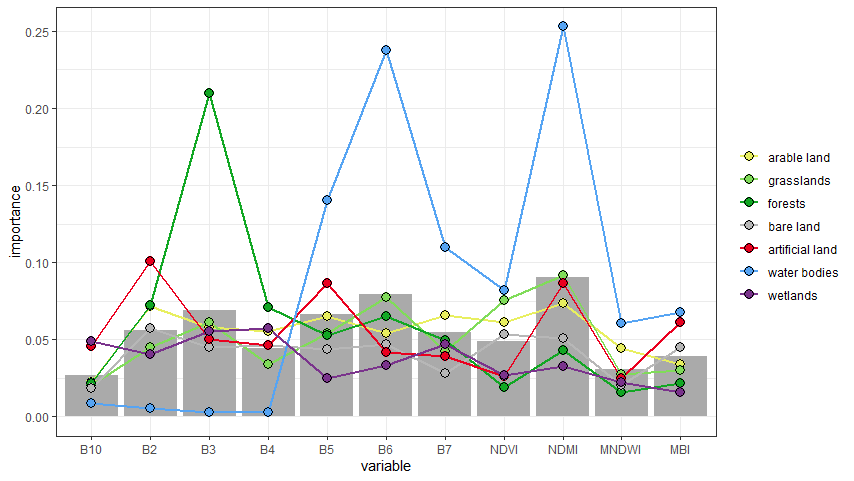
\includegraphics[width=5.59375in,height=3.125in]{./figures/importance_comparison.png}

}

\caption{\label{fig-rycina14a}Comparison of variable importance values
by land cover class and variable. Grey bars show average value of
importance of a variable.}

\end{figure}

In the last step of evaluating thermal band's importance for the model,
I created partial-dependence (PD) profiles for this variable
(Figure~\ref{fig-rycina15}) and compared it with PD profile for
near-infrared band (B5) presented in Figure~\ref{fig-rycina16}. Thanks
to PD plots, I checked how probability for choosing certain class
changed with increasing values of analysed variables while keeping other
features at their average values. Probabilities do not drastically
change with temperature (thermal band's value) increase, there are only
small fluctuations for several classes. This allows us to conclude that
thermal band might not have significant impact on model results. In
contrast, B5 variable profile has clearly visible fluctuations for
nearly every class (Figure~\ref{fig-rycina16}). Probabilities change
significantly along with changes of near-infrared values, thus
suggesting that this variable has greater impact on the model
predictions than thermal band.

\begin{figure}[H]

{\centering 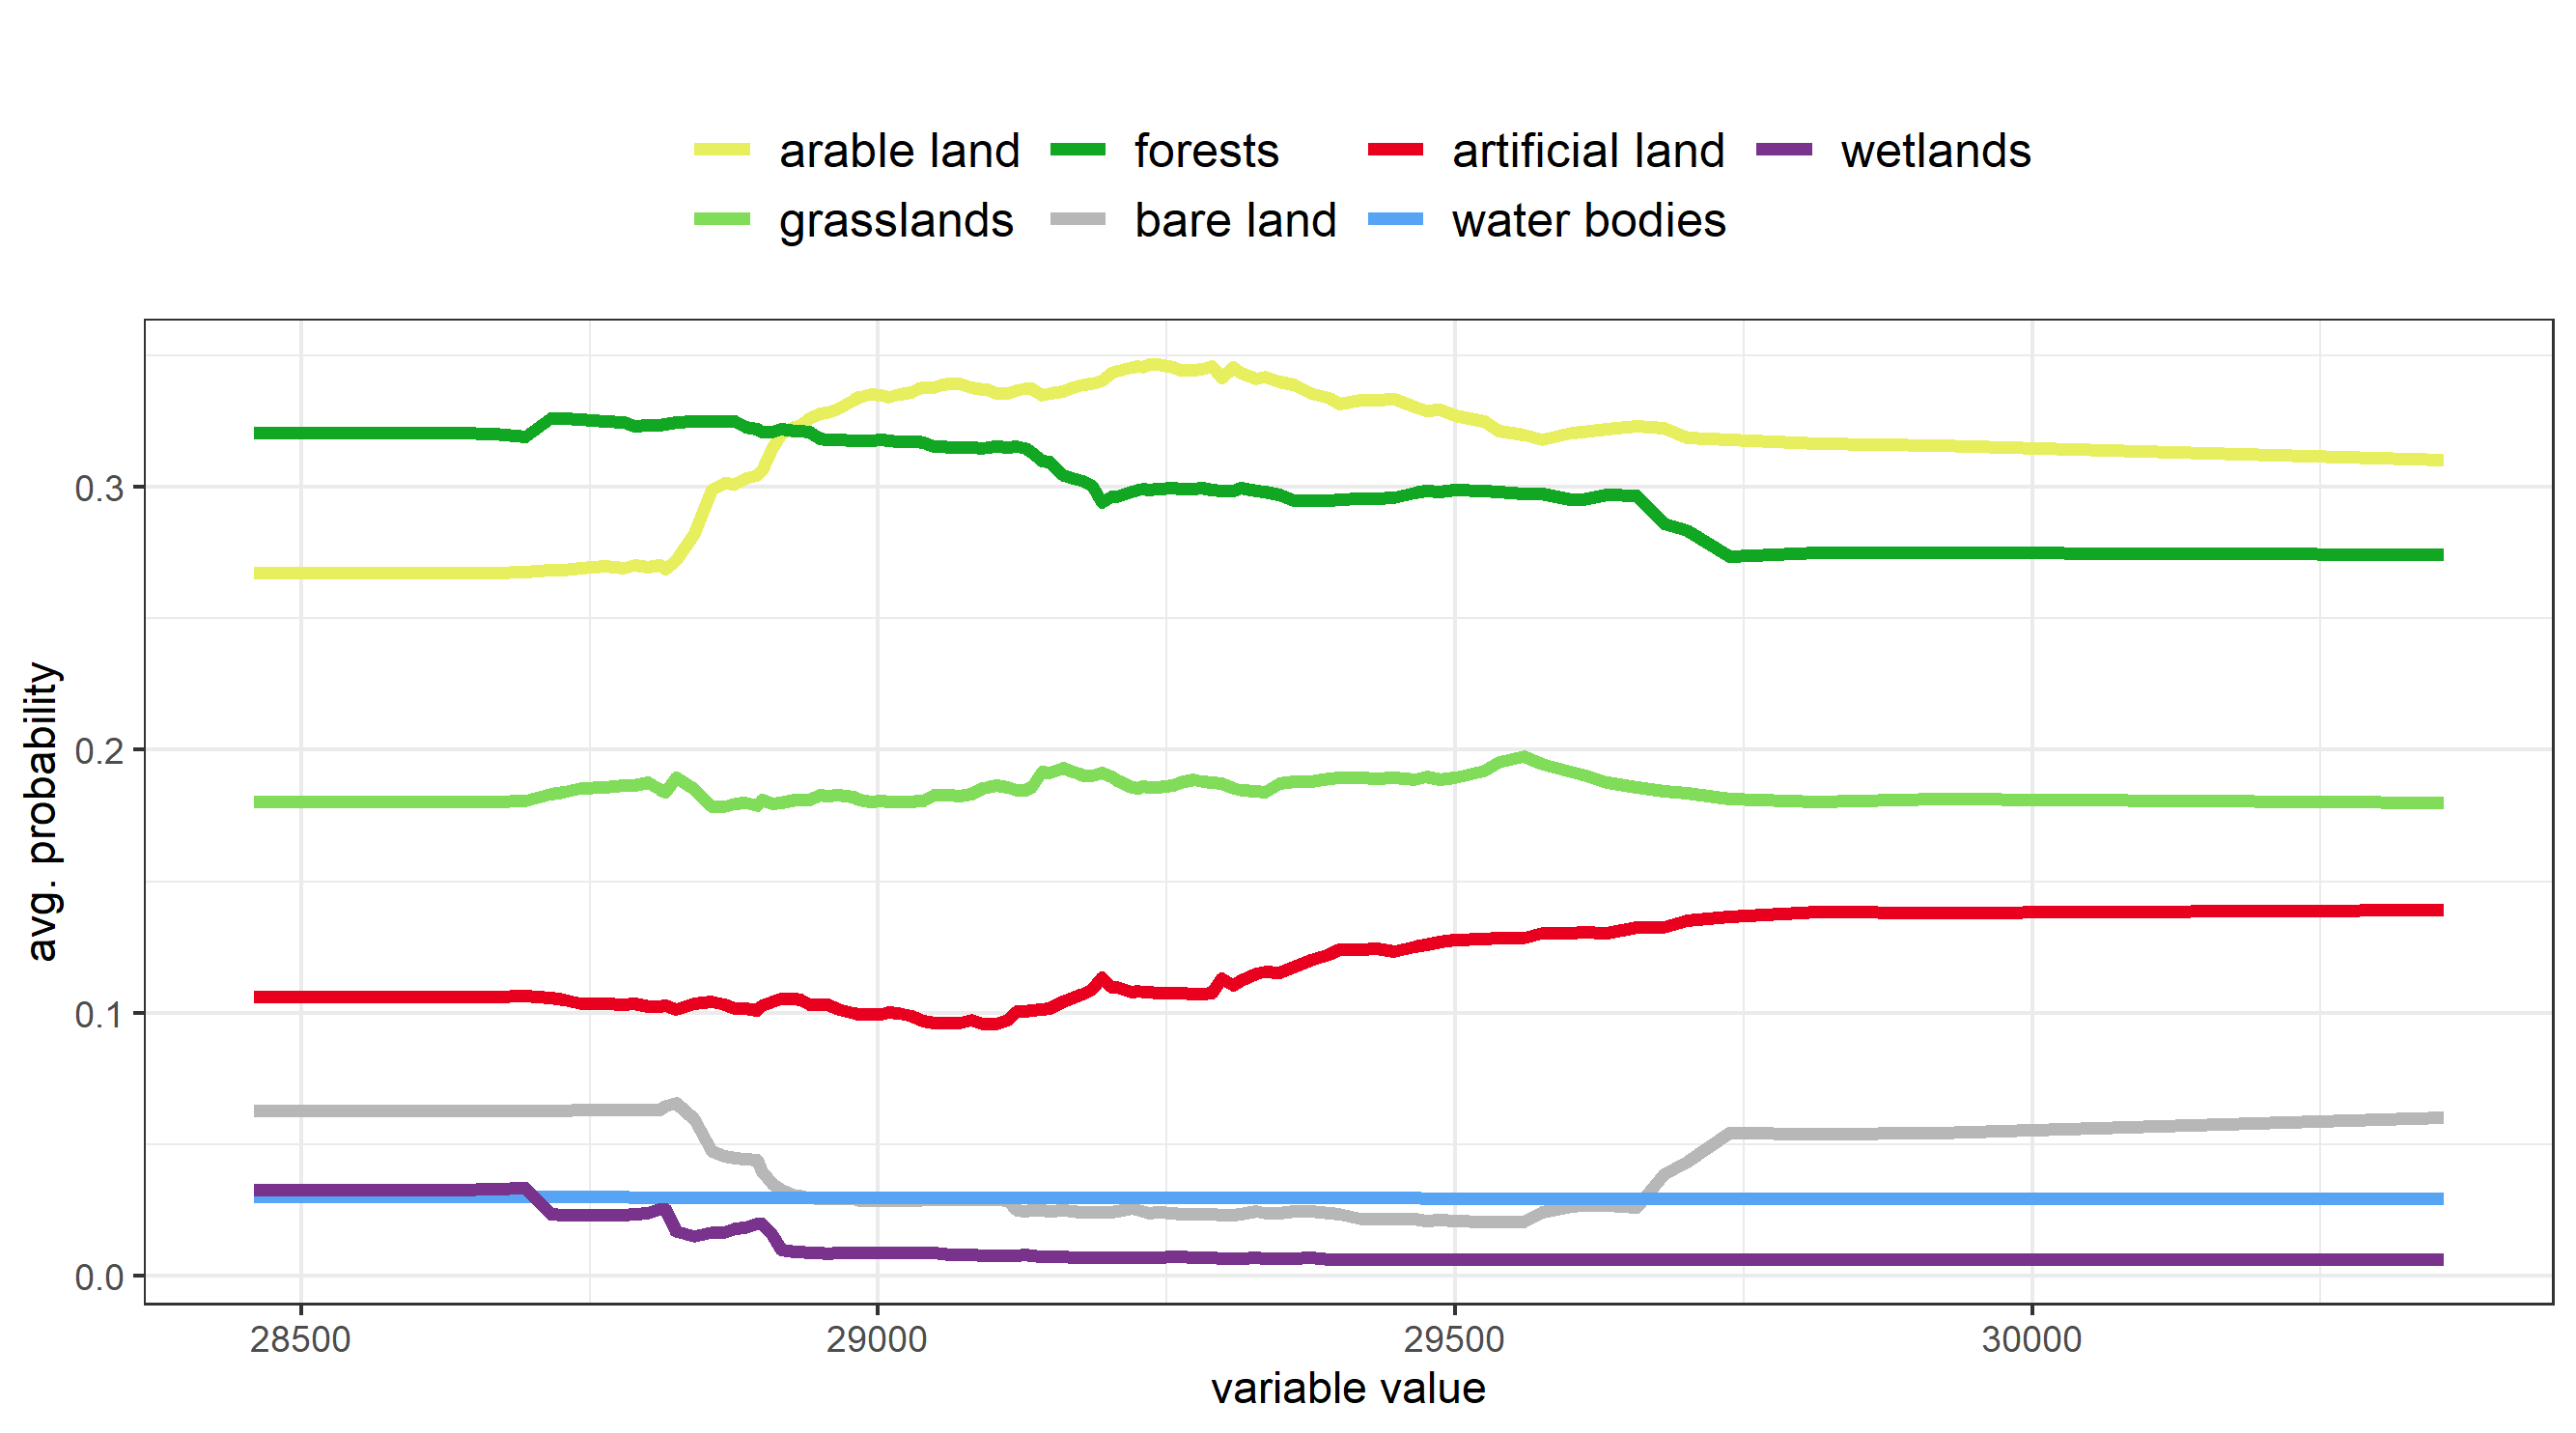
\includegraphics[width=5.625in,height=3.125in]{./figures/profB10.png}

}

\caption{\label{fig-rycina15}Partial-dependence profile for thermal band
(B10)}

\end{figure}

\begin{figure}[H]

{\centering 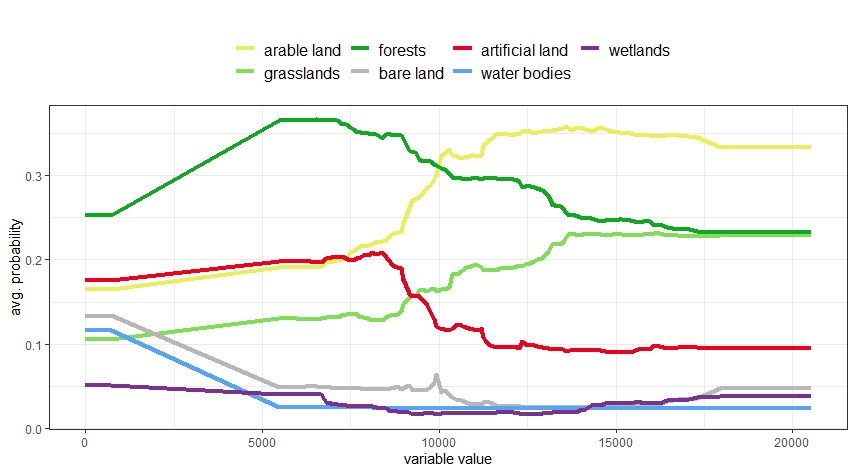
\includegraphics[width=5.625in,height=3.125in]{./figures/profB5.png}

}

\caption{\label{fig-rycina16}Partial-dependence profile for
near-infrared band (B5)}

\end{figure}

\hypertarget{sec-imp-spat}{%
\section{Spatial distribution of thermal band's
importance}\label{sec-imp-spat}}

Variable importance values computed for LUCAS points in
Section~\ref{sec-imp-overall} were used to interpolate them into
continuous raster layer using IDW interpolation method. This step
created an opportunity to examine approximate spatial distribution of
thermal band's importance across Poznań metropolitan area
(Figure~\ref{fig-rycina17}).

\begin{figure}[H]

{\centering 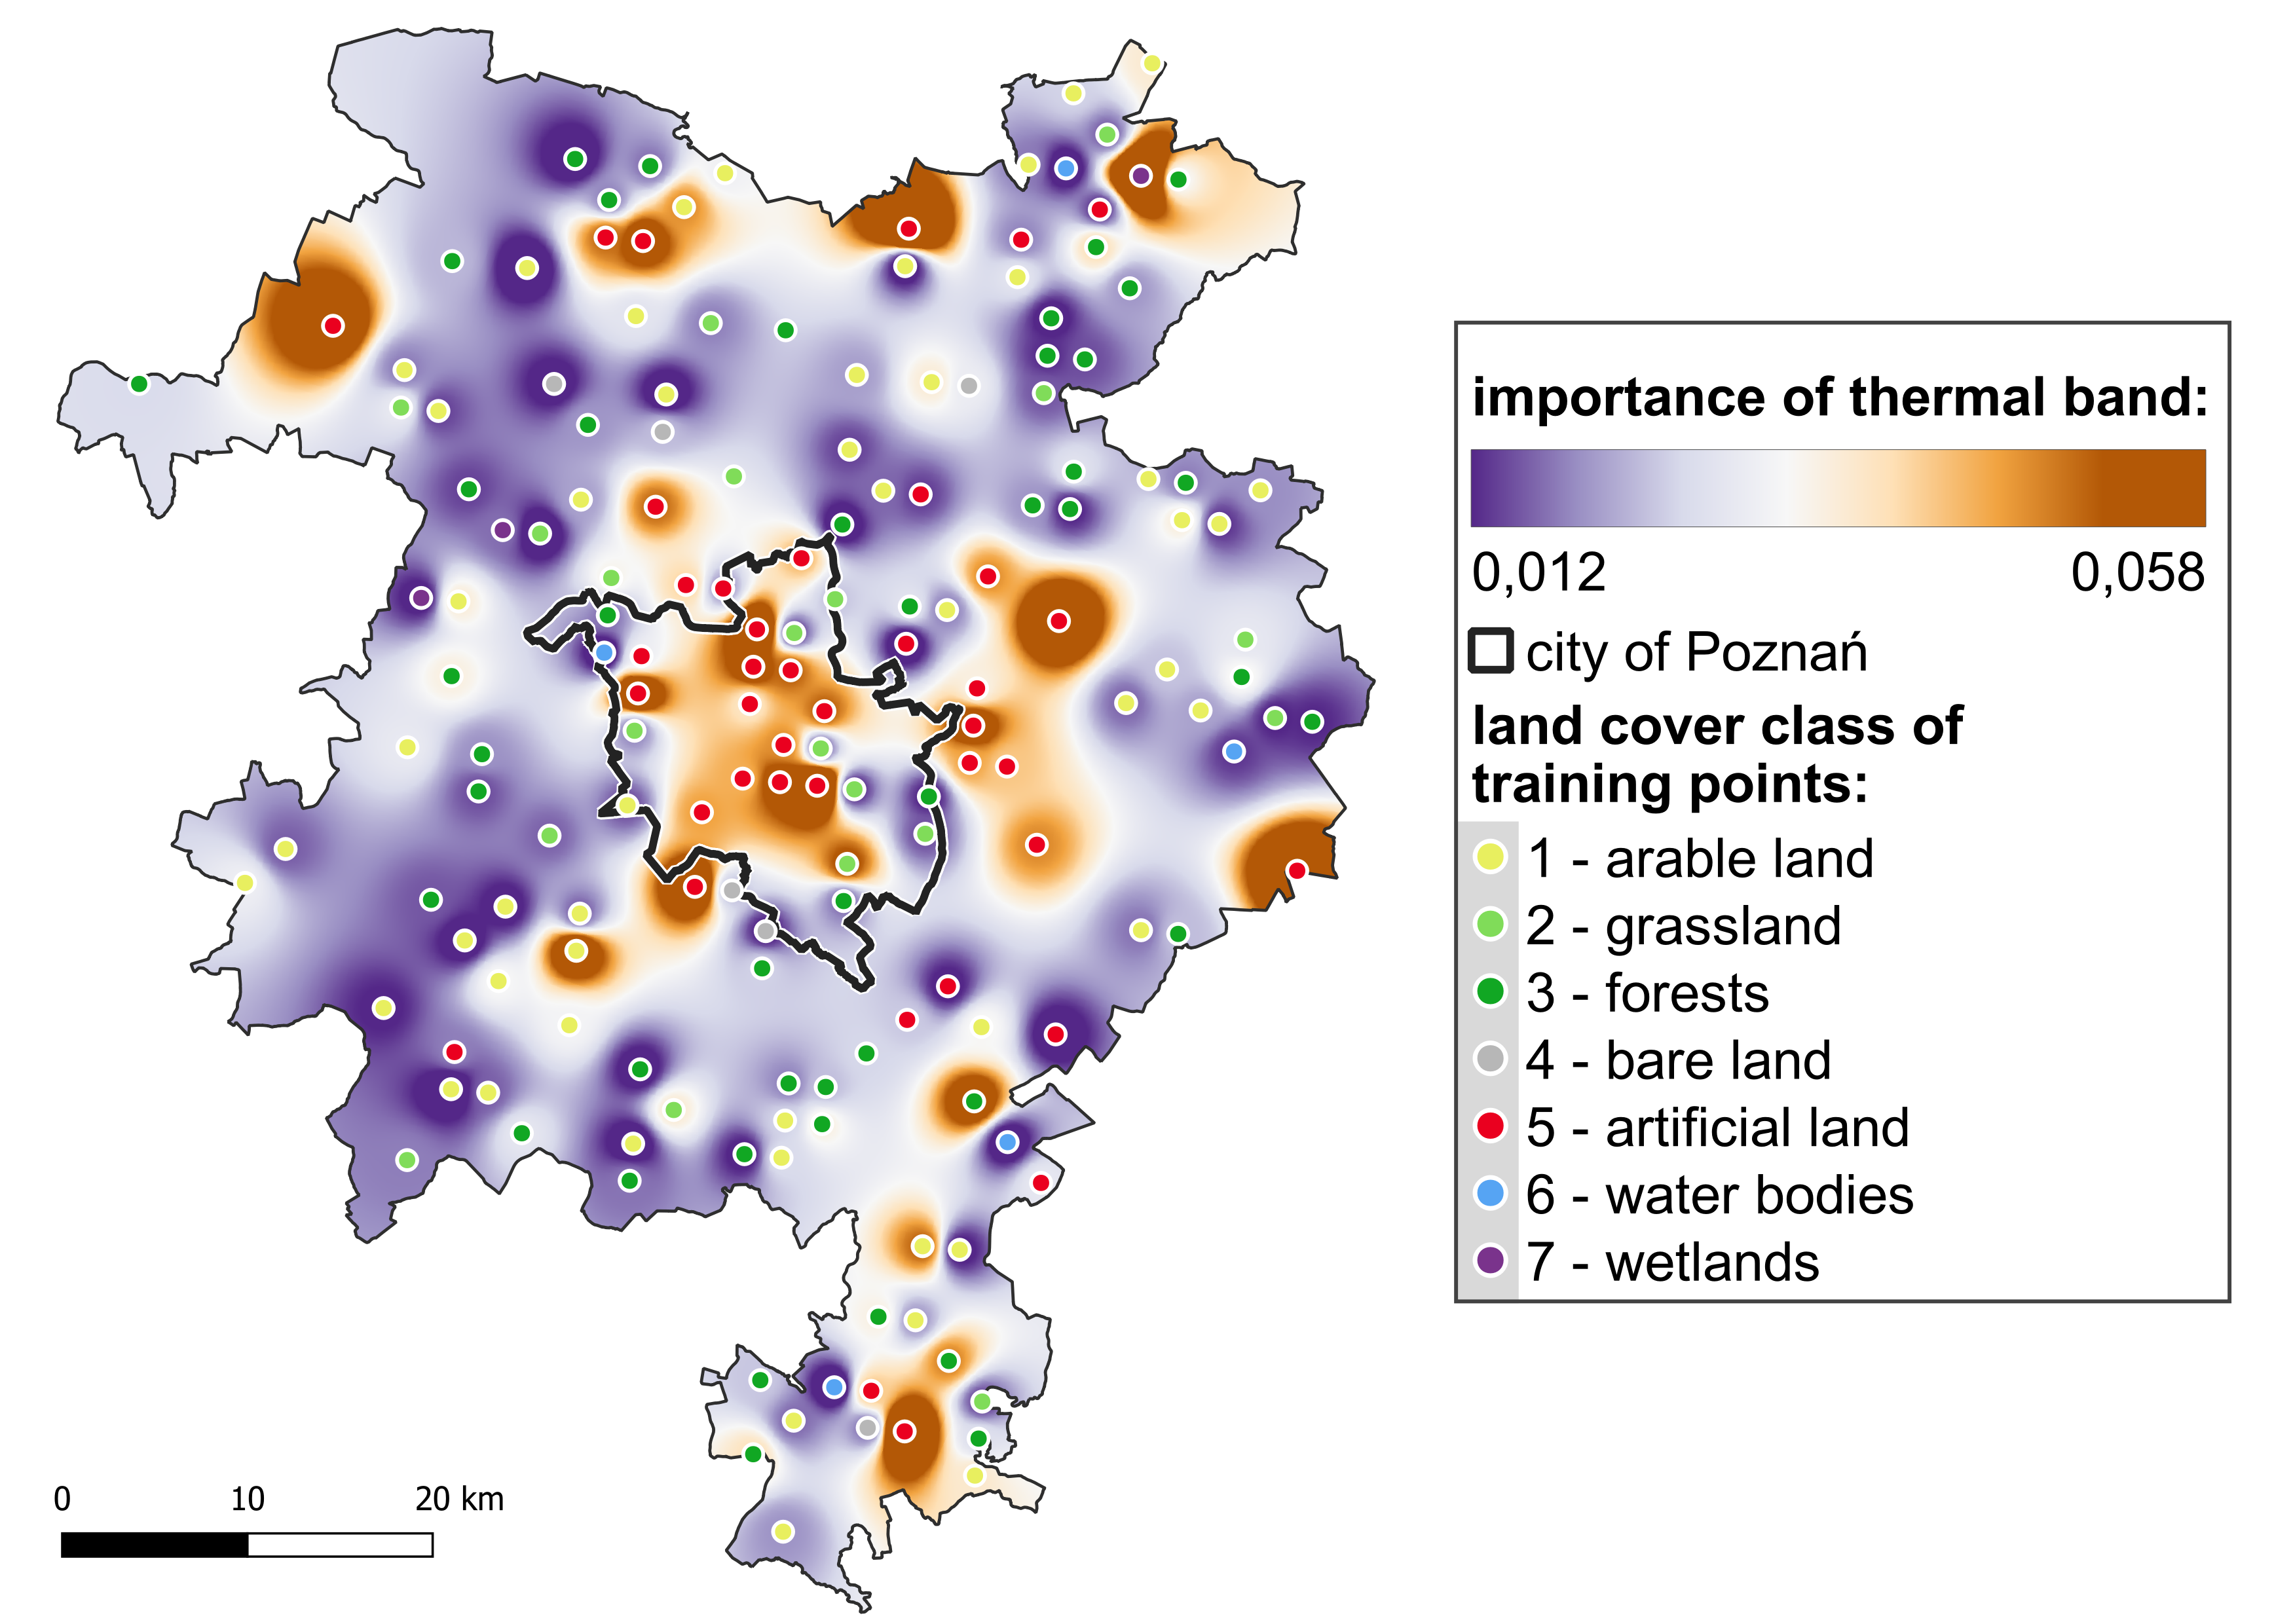
\includegraphics[width=5.875in,height=4.16667in]{./figures/B10_importance-spatial-ENG.png}

}

\caption{\label{fig-rycina17}Thermal band importance interpolated from
values on LUCAS points locations}

\end{figure}

Moreover, alternative approach involving raster aggregation was also
implemented. In this method, original satellite data was aggregated
(resampled) to 1,5 km resolution in order to make analysis more general
and to shorten the computation time. After aggregation, thermal band's
importance was calculated for every raster cell. Result of these
calculations, as well as aggregated raster in RGB composition, are shown
in Figure~\ref{fig-rycina18}. In general, there is similar distribution
of thermal band's importance like in Figure~\ref{fig-rycina17}, however
this approach does not require interpolation of values from points which
may be misleading, especially in places far away from LUCAS points. On
the other hand, spectral values were averaged for every 1,5 km cell so
these mean values may not represent accurately features on the ground.

\begin{figure}[H]

{\centering 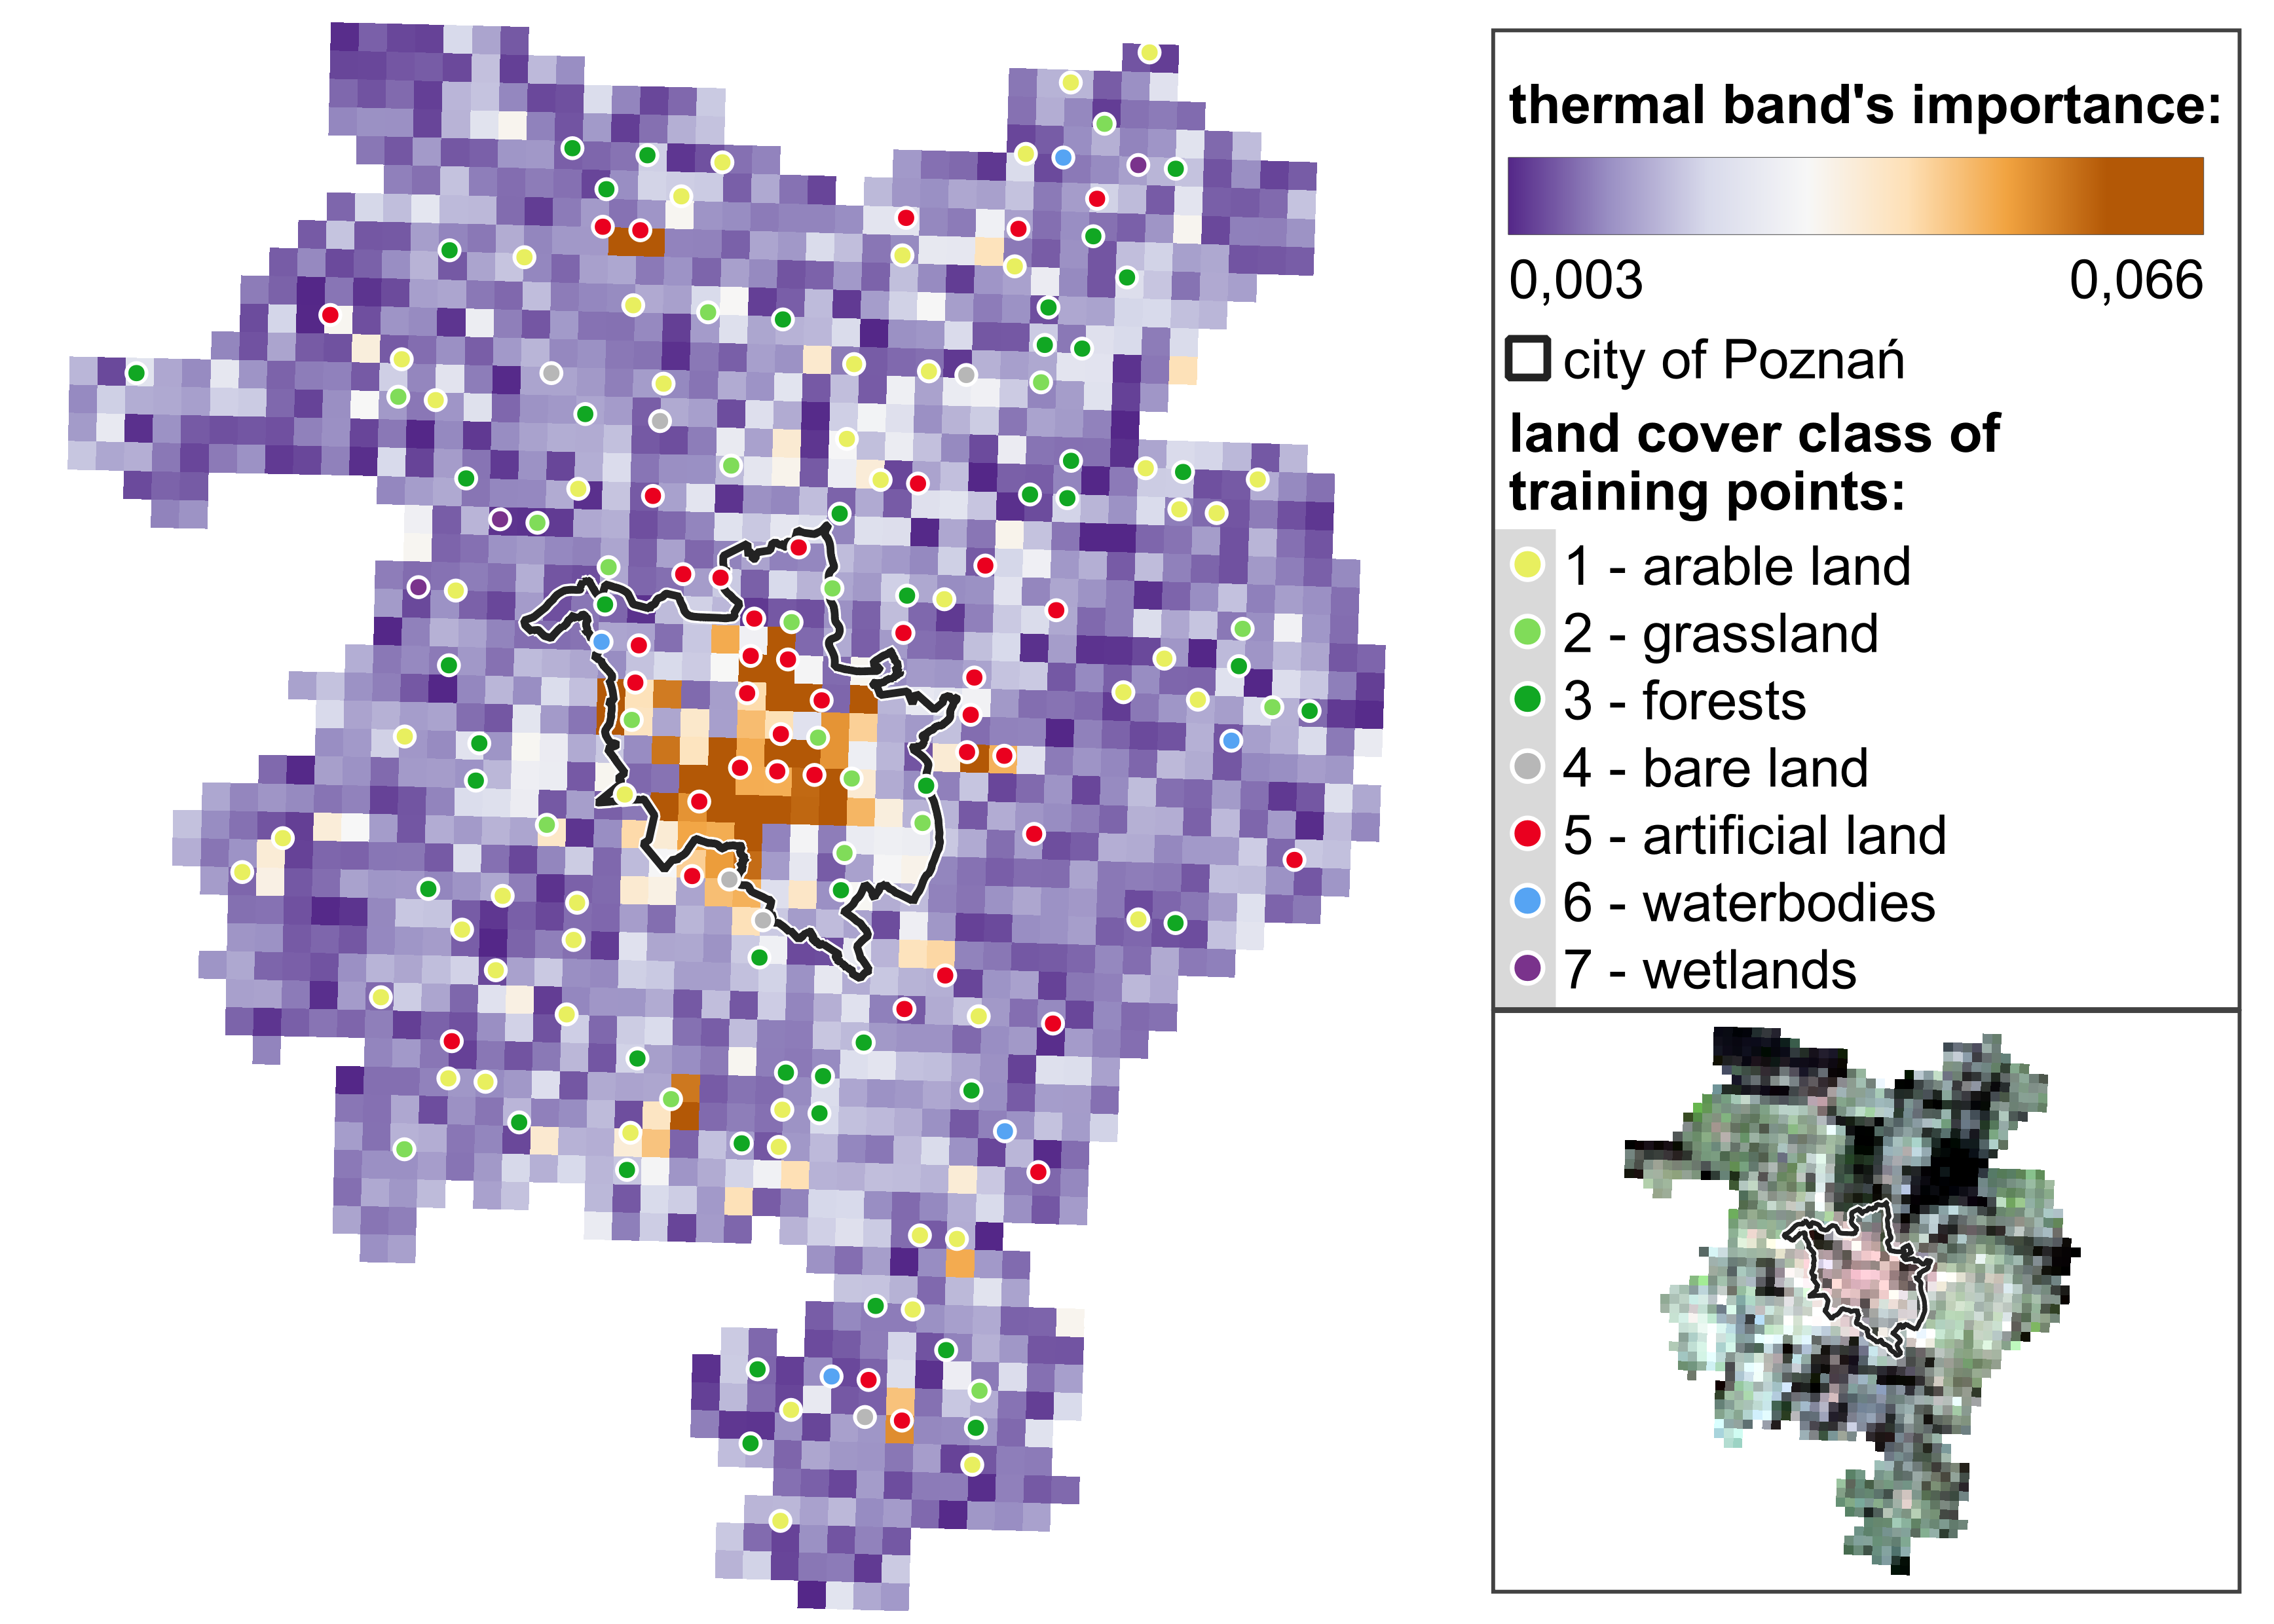
\includegraphics[width=5.875in,height=4.16667in]{./figures/B10_importance-spatial-ENG2.png}

}

\caption{\label{fig-rycina18}Thermal band importance calculated for
raster cells aggregated to 1,5 km resolution. Small map in right-bottom
corner shows averaged spectral values in RGB composition.}

\end{figure}

Correlation of thermal band's importance with artificial land class is
visible on both maps. In each case, high importance values are
concentrated mainly in urban areas, especially in Poznań as it is the
biggest city in the study area. Also in smaller towns there is a higher
thermal band's impact on model results, but because of their size, it is
often harder to detect.

\bookmarksetup{startatroot}

\hypertarget{conclusion}{%
\chapter{Conclusions}\label{conclusion}}

This study showed that thermal band's impact on machine learning model
results is not very strong overall and quantifying its importance needs
more in-depth approach. The land cover map was created from imagery of
only one 16-day interval and its accuracy was rather average, especially
when compared with state-of-the-art works in this field
\autocite{malinowski_automated_2020,witjes_spatiotemporal_2021}. On the
other hand, obtained results were accurate enough to apply methods of
measuring variable importance and to make some conclusions from findings
of this analysis.

In order to add spatial context to the importance values, two methods of
creating variable importance maps were developed in my work. The first
method applied points interpolation, while the second one used raster
aggregation and averaged spectral values. After analysis of the created
maps, it became clear that thermal band was more influential in
classifying urban areas than for rest of the classes, although its
importance was mostly correlated with land cover type. Clear
spatial-autocorrelation of thermal band's importance was not detected,
probably because of too sparsely distributed training points. Above
method should be further examined and tested, since studying spatial
distribution of variable importance could improve our understanding of
different variables' impact on machine learning model results or may
provide new knowledge in this topic.

The most substantial difference between this work and previous studies
on the topic is the scope of variable importance evaluation. Both
Rodríguez-Galiano et al.
\autocite*{rodriguez-galiano_incorporating_2012} and Zhao
\autocite*{zhao_exploring_2019} used only variable importance estimation
built into the Random Forest algorithm. Sun and Shulz
\autocite*{sun_improvement_2015} analysed an increase of overall
accuracy (OA) of the model only. In contrast, variable importance was
evaluated in this study using several methods such as permutation-based
computation, break-down plots, Shapley values and partial-dependence
profiles (Section~\ref{sec-importance}). All these approaches gave
similar outcomes - thermal band had low impact on the general results of
the created model. Inclusion of thermal band increased overall
performance measures by a very narrow margin (less than 1\%), which is
not as optimistic outcome as in previously mentioned studies
\autocite{rodriguez-galiano_incorporating_2012,sun_improvement_2015,zhao_exploring_2019}.
All these works estimated impact of thermal band on overall accuracy at
2-10\%. However, more in-depth analysis revealed that land surface
temperature had greater impact on predicting artificial land than any
other land cover class. Also Rodríguez-Galiano et al.
\autocite*{rodriguez-galiano_incorporating_2012} and Zhao
\autocite*{zhao_exploring_2019} discovered that thermal band improves
classification of artificial areas. On the other hand, my results does
not confirm other finding of Zhao \autocite*{zhao_exploring_2019},
stating that thermal band helps in distinguishing arable land from
wetlands - this divergence is probably caused by entirely different
environments of study areas, Egypt and Poland.

Findings of my study suggest that thermal band could help in mapping the
development of cities and urban areas. Its inclusion may help
distinguish an artificial land from other similar land cover types. More
accurate land cover maps will help in better growth management of
metropolitan areas and in quantifying impact of urbanization on natural
environment more precisely. Nonetheless, further research should be
carried out on bigger area and for larger number of satellite images. It
is crucial to extend this study to include spatio-temporal aspect of
imagery, in order to investigate thermal band's impact on model
predictions throughout different vegetation seasons. Moreover, areas
from different climate zones should be examined with an emphasis on the
thermal band importance issue. Newly launched Landsat 9 satellite can
also provide improvement for thermal band's use for land cover mapping,
because its thermal sensor is expected to perform better in Earth
observation than its predecessor from Landsat 8.

\printbibliography[heading=bibintoc, title=Bibliography]

\end{document}
